\documentclass[aspectratio=169, 10pt]{beamer}

%Packages
\usepackage[utf8]{inputenc}
\usepackage{amsmath}
\usepackage{amsfonts}
\usepackage{amssymb}
% \usepackage{algorithm2e}
% \usepackage{algorithmic}
\usepackage{listings}
\usepackage{xcolor}
\usepackage{tikz}
\usepackage{hyperref}
\usepackage{algorithm}
\usepackage{algpseudocode}
\usepackage{booktabs}
\usepackage{bm}
% Setup for code appearance
\renewcommand{\algorithmicrequire}{\textbf{Input:}}
\renewcommand{\algorithmicensure}{\textbf{Output:}}
\algnewcommand{\LineComment}[1]{\Statex \(\triangleright\) #1}
\graphicspath{{../analysis/plots/}{images/}}
\usepackage[backend=bibtex,style=numeric]{biblatex}
\addbibresource{refs}
%just a comment
% =========================
% THEME & COLORS (Black Background)
% =========================
\definecolor{bgblack}{RGB}{0,0,0}
\definecolor{fgwhite}{RGB}{240,240,240}
\definecolor{accentcyan}{RGB}{0, 255, 255}
\definecolor{softgray}{RGB}{100,100,100}
\definecolor{codebg}{RGB}{20,20,20}
\definecolor{codegreen}{RGB}{0,200,100}
\definecolor{codeblue}{RGB}{80,160,255}
\definecolor{codepurple}{RGB}{200,100,255}
\usepackage{subcaption}
\setbeamercolor{background canvas}{bg=bgblack}
\setbeamercolor{normal text}{fg=fgwhite}
\setbeamercolor{frametitle}{fg=accentcyan}
\setbeamercolor{title}{fg=accentcyan}
\setbeamercolor{structure}{fg=accentcyan}
\setbeamercolor{item}{fg=accentcyan}
\setbeamercolor{section in toc}{fg=fgwhite}
\setbeamercolor{subsection in toc}{fg=fgwhite}
\setbeamercolor{footnote}{fg=fgwhite}
\setbeamercolor{footnote mark}{fg=accentcyan}
% Make main text slightly smaller for a more compact layout
% (reduce global font a bit without changing documentclass option)
\setbeamerfont{normal text}{size=\small}
\setbeamerfont{frametitle}{size=\small}
\setbeamerfont{title}{size=\small}
\setbeamerfont{author}{size=\small}
\setbeamerfont{institute}{size=\scriptsize}

% Listings setup for LAMMPS/Python code
\lstset{
    backgroundcolor=\color{codebg},
    basicstyle=\ttfamily\footnotesize\color{fgwhite},
    commentstyle=\color{softgray},
    keywordstyle=\color{codepurple},
    numberstyle=\footnotesize\color{softgray},
    stringstyle=\color{codegreen},
    breaklines=true,
    frame=leftline,
    rulecolor=\color{accentcyan},
    numbers=left,
    xleftmargin=10pt,
}

% Title Info
\title{Solvent Structure around Nanoparticles}
\subtitle{Investigating Hydrophobicity via MD Simulations and analysis using ML}
\author{\href{https://shuvam-banerji-seal.github.io/}{Shuvam Banerji Seal} (22MS076)}
\institute{Indian Institute of Science Education and Research Kolkata}
\date{\today}

\begin{document}

% =========================
% SLIDE 1: Title
% =========================
\begin{frame}
    % \centering
    % \Huge \textbf{\textcolor{accentcyan}{Solvent Structure around Nanoparticles}} \\
    % \vspace{0.5cm}
    % \large Tuning Hydrophobicity \& Hydrophilicity \\
    % \vspace{1cm}
    % \normalsize \textbf{Shuvam Banerji Seal} \\
    % \scriptsize \url{https://shuvam-banerji-seal.github.io/} \\
    % \vspace{0.5cm}

    \titlepage
    \scriptsize Repository: \url{git@github.com:Shuvam-Banerji-Seal/Solvent-Structure-around-NanoParticles.git}
\end{frame}

% =========================
% SLIDE 2: TOC
% =========================
\begin{frame}[allowframebreaks]{Table of Contents}
    \tableofcontents
\end{frame}
\begin{frame}{What did I contribute to the society by doing this project?}

    \pause 
    \centering
    \Large \textbf{Well there are 3 things...}
    \pause
    \newline
    Let's explore then one by one   
\end{frame}
\begin{frame}{My Contributions to Society}

\centering
Creating the \href{https://shuvam-banerji-seal.github.io/lammps_data_web_viewer/}{Online Lammps Molecule Viewer}

    \begin{figure}
        \centering
        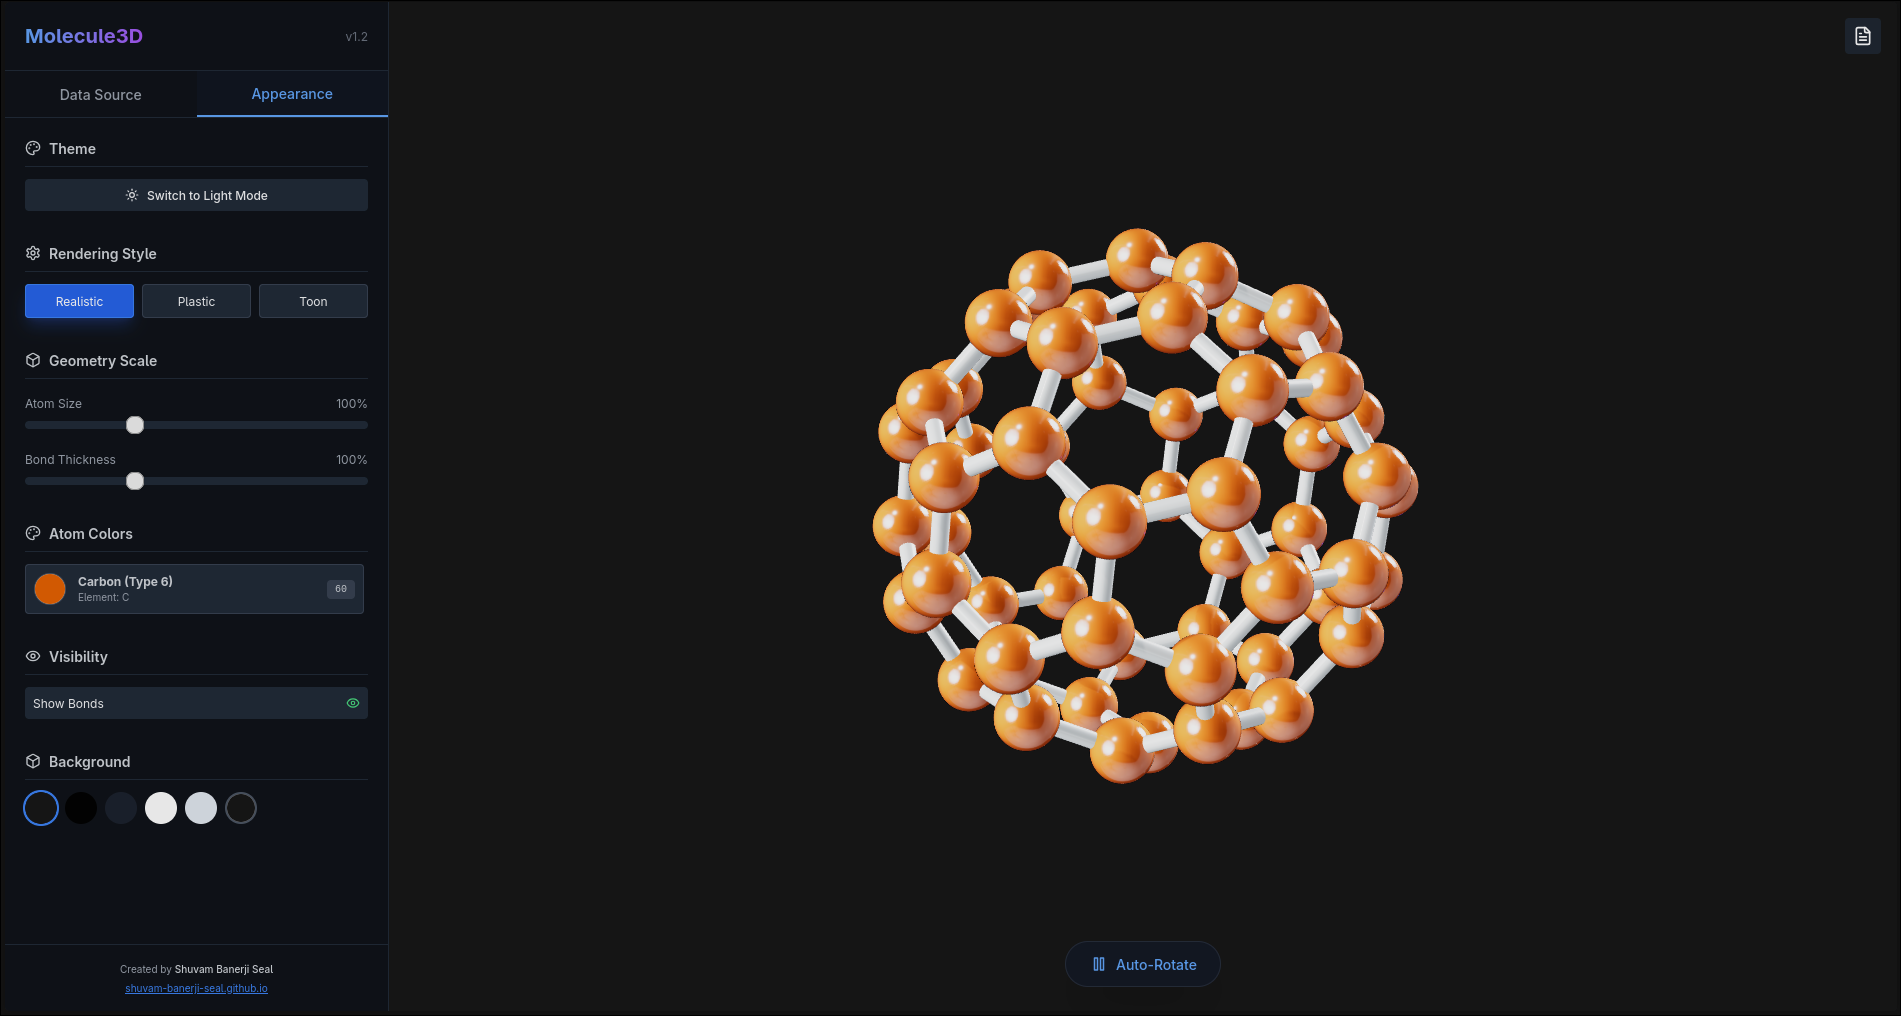
\includegraphics[width=0.8\linewidth]{images/lammps_webview.png}
        \caption{\url{https://shuvam-banerji-seal.github.io/lammps_data_web_viewer/ }}
        \label{fig:placeholder}
    \end{figure}
\end{frame}

    
% =========================
% SECTION: Intro
% =========================
\section{Introduction}
\subsection{Problem Statement}

\begin{frame}{Problem Statement}
    \begin{columns}
        \column{0.6\textwidth}
        \textbf{Core Scientific Question:}
        \begin{itemize}
            \item How does the solvent (water) reorganize itself around a nanoparticle (C60)?
            \item How does this reorganization change as we tune the interaction strength ($\epsilon_{CO}$)?
            \item \textit{Hypothesis:} The transition from hydrophobic to hydrophilic induces a structural phase transition in the solvation shell.
        \end{itemize}
        
        \vspace{0.5cm}
        \textbf{The Machine Learning Angle:}
        \begin{itemize}
            \item Can we generate descriptors (RDF fingerprints, Voronoi tessellation) from MD trajectories?
            \item Can ML models predict aggregation propensity based purely on local solvent structure?
        \end{itemize}

        \column{0.4\textwidth}
        \centering
        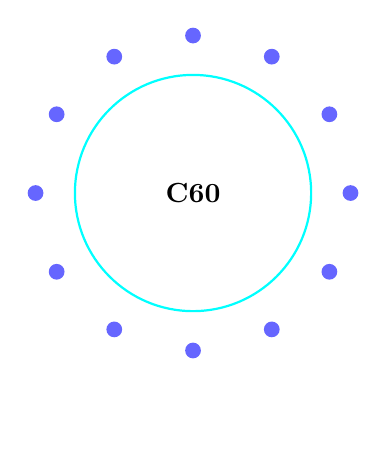
\begin{tikzpicture}
            \draw[accentcyan, thick] (0,0) circle (1.5cm);
            \node at (0,0) {\textbf{C60}};
            \foreach \angle in {0,30,...,330}
                \fill[blue!60] (\angle:2cm) circle (0.1cm);
             \node[below, white] at (0,-2.5) {Solvation Shell};
        \end{tikzpicture}
    \end{columns}
\end{frame}

% =========================
% SECTION: System Overview
% =========================
\section{System Overview}
\subsection{Simulation Setup}

\begin{frame}{The Simulated System}
    \textbf{Composition:}
    \begin{itemize}
        \item \textbf{Solute:} 3 $\times$ Buckminsterfullerene (C60) Molecules ($N_{atoms} = 180$).
        \item \textbf{Solvent:} $\sim$2000 Water molecules (TIP4P/2005 model) \footfullcite{abascal2005general}.
        \item \textbf{Box:} Cubic $40 \times 40 \times 40$ \AA$^3$ (Periodic Boundary Conditions).
    \end{itemize}

    \vspace{0.5cm}
    \textbf{Physics Engine (LAMMPS) \footfullcite{thompson2022lammps}:}
    \begin{itemize}
        \item \textbf{Force Field:} Lennard-Jones + Coulombic (Long Range).
        \item \textbf{Thermostat/Barostat:} Nosé-Hoover (NVT/NPT) \footfullcite{nose1984unified, hoover1985canonical}.
        \item \textbf{Constraints:} SHAKE algorithm for rigid water bonds \footfullcite{ryckaert1977numerical}.
    \end{itemize}
\end{frame}

% =========================
% SECTION: Methodology - Files
% =========================
\section{Methodology}
\subsection{System Construction}

\begin{frame}{Step 1: Raw Data (\texttt{C60.data})}
    \textbf{Origin:} 
    Derived from the standard XYZ coordinates available in the LAMMPS library.
    
    \vspace{0.5cm}
    \textbf{Content:}
    \begin{itemize}
        \item Contains spatial coordinates $(x, y, z)$ for 60 Carbon atoms.
        \item \textit{Limitation:} Purely geometric. No bonding topology (bonds, angles, dihedrals) is defined in the raw file.
    \end{itemize}
    
    \vspace{0.5cm}
    \textit{We must computationally infer the topology to treat C60 as a rigid, bonded molecule.}
\end{frame}

% =========================
% TOPOLOGY GENERATION
% =========================
\begin{frame}[fragile]{Step 2: Topology Generation (\texttt{generate\_C60\_bonded.py})}
    \textbf{Objective:} Transform point cloud to bonded graph.
    \textbf{Bond Criteria:} C-C bond length in Fullerene $\approx 1.4$ \AA. Threshold: $1.3 \le r_{ij} \le 1.5$ \AA.

    \begin{columns}
    \column{0.5\textwidth}
    \begin{algorithmic}[1]
        \State Read Atoms $A = \{a_1, ..., a_{60}\}$
        \State $Bonds \leftarrow []$
        \For{$i \in 1 \dots 60$}
            \For{$j \in (i+1) \dots 60$}
                \State $d_{ij} = \sqrt{(x_i-x_j)^2 + ...}$
                \If{$1.3 \le d_{ij} \le 1.5$}
                    \State $Bonds.append((i, j))$
                \EndIf
            \EndFor
        \EndFor
        \State \textbf{Verify:} Count bonds per atom
        \If{$\forall i, Count(i) == 3$}
            \State Write \texttt{C60\_bonded.data}
        \Else
            \State \textbf{Error:} Invalid Topology
        \EndIf
    \end{algorithmic}
    
    \column{0.5\textwidth}
    \textbf{Mathematical Basis:}
    Euclidean Distance Metric:
    \begin{equation}
        r_{ij} = ||\mathbf{r}_i - \mathbf{r}_j||_2
    \end{equation}
    Graph Theory Constraint:
    \begin{equation}
        deg(v) = 3, \quad \forall v \in V_{C60}
    \end{equation}
    Total Bonds:
    \begin{equation}
        |E| = \frac{1}{2} \sum deg(v) = \frac{60 \times 3}{2} = 90
    \end{equation}
    \end{columns}
\end{frame}

% =====================================================================
% SECTION: Detailed Script Analysis - Validation
% =====================================================================
\subsection{Validation}

% --- Slide: Initialization & Potentials ---
\begin{frame}[fragile]{Validation Script: Initialization \& Force Field}
    \textbf{1. Atom Definition:}
    \begin{lstlisting}[language=bash]
    units real          # Energy: kcal/mol, Dist: Angstrom, Time: fs
    atom_style full     # Attributes: ID Mol Type Charge X Y Z
    \end{lstlisting}
    \textit{Physics:} `full` is required because TIP4P water relies on partial charges ($q_O = -1.04e, q_H = +0.52e$).

    \vspace{0.3cm}
    \textbf{2. TIP4P/2005 Pair Style:}
    \begin{lstlisting}[language=bash]
    pair_style lj/cut/tip4p/long/omp 2 3 2 1 0.1546 12.0
    \end{lstlisting}
    \textit{Mathematical Model:} The potential includes a virtual site $M$ located $d_{OM} = 0.1546$\AA\ from Oxygen along the H-O-H bisector.
    \begin{equation}
        \mathbf{r}_M = \mathbf{r}_O + d_{OM} \frac{\mathbf{r}_{H1} + \mathbf{r}_{H2} - 2\mathbf{r}_O}{||\mathbf{r}_{H1} + \mathbf{r}_{H2} - 2\mathbf{r}_O||}
    \end{equation}
    The interaction energy is:
    \begin{equation}
        U_{ij} = 4\epsilon_{ij} \left[ \left(\frac{\sigma_{ij}}{r_{ij}}\right)^{12} - \left(\frac{\sigma_{ij}}{r_{ij}}\right)^6 \right] + \frac{q_M q_{j}}{4\pi\epsilon_0 r_{Mj}}
    \end{equation}
\end{frame}

% --- Slide: Bonding & Topology ---
\begin{frame}[fragile]{Validation Script: Topology \& Harmonics}
    \textbf{3. Reading Topology:}
    \begin{lstlisting}[language=bash]
    read_data C60_bonded.data add merge
    molecule h2omol H2O_TIP4P2005_fixed.mol offset 1 1 0 0 0
    \end{lstlisting}
    \textit{Logic:} Merges the C60 graph with the rigid water template.

    \vspace{0.3cm}
    \textbf{4. Bonded Potentials (Harmonic Approximation):}
    \begin{lstlisting}[language=bash]
    bond_style harmonic  ; bond_coeff 1 938.0 1.42
    angle_style harmonic ; angle_coeff 1 0.0 104.52
    \end{lstlisting}
    \textit{Equation:} For C60 C-C bonds ($k_b = 938$ kcal/mol/\AA$^2$):
    \begin{equation}
        U_{bond}(r) = K_b (r - r_0)^2
    \end{equation}
    Note: Water bond coeffs are set to 0.0 because we use SHAKE (next slide).
\end{frame}

% --- Slide: SHAKE Constraints ---
\begin{frame}[fragile]{Validation Script: The SHAKE Algorithm}
    \textbf{5. Constraint Application:}
    \begin{lstlisting}[language=bash]
    fix water_shake water_group shake 0.0001 20 0 b 2 a 1
    \end{lstlisting}
    
    \textbf{Mathematical Detail:}
    We treat water as a rigid body. Instead of solving Newton's equations directly, we solve the constrained Lagrangian:
    \begin{equation}
        \mathcal{L} = \sum \frac{1}{2} m_i \dot{\mathbf{r}}_i^2 - V(\mathbf{r}) - \sum_{k} \lambda_k \sigma_k(\mathbf{r})
    \end{equation}
    Where the holonomic constraints $\sigma_k$ are:
    \begin{equation}
        \sigma_{OH} = ||\mathbf{r}_O - \mathbf{r}_H||^2 - d_{OH}^2 = 0
    \end{equation}
    \textbf{Algorithm:}
    LAMMPS iteratively updates positions $\mathbf{r}(t+\delta t)$ until the constraints are satisfied within tolerance ($10^{-4}$).
\end{frame}

% --- Slide: Dynamics (NVT) ---
\begin{frame}[fragile]{Validation Script: Time Integration (NVT)}
    \textbf{6. Thermostatting:}
    \begin{lstlisting}[language=bash]
    velocity all create 300 12345 dist gaussian
    fix 1 water_group nvt temp 300 300 100.0
    \end{lstlisting}

    \textbf{Nosé-Hoover Equations of Motion:}
    The code integrates these coupled differential equations:
    \begin{align}
        \dot{\mathbf{r}}_i &= \frac{\mathbf{p}_i}{m_i} \\
        \dot{\mathbf{p}}_i &= \mathbf{F}_i - \zeta \mathbf{p}_i \\
        \dot{\zeta} &= \frac{1}{Q} \left( \sum \frac{\mathbf{p}_i^2}{m_i} - (3N+1)k_B T_{target} \right)
    \end{align}
    where $\zeta$ is the friction variable and $Q$ is the thermal inertia parameter (controlled by `Tdamp = 100.0`) \footfullcite{nose1984unified}.
\end{frame}

% --- Slide: Validation Metric ---
\begin{frame}[fragile]{Validation Script: Radius of Gyration}
    \textbf{7. Structural Integrity Check:}
    \begin{lstlisting}[language=bash]
    compute rg_c60_compute c60_group gyration
    fix rg_output all print 100 ...
    \end{lstlisting}

    \textbf{Metric Definition:}
    To ensure the C60 doesn't collapse or explode, we calculate the scalar Radius of Gyration $R_g$:
    \begin{equation}
        R_g = \sqrt{ \frac{1}{M} \sum_{i=1}^{60} m_i (\mathbf{r}_i - \mathbf{r}_{COM}) \cdot (\mathbf{r}_i - \mathbf{r}_{COM}) }
    \end{equation}
    \textbf{Success Criteria:} For C60, $R_g$ must remain strictly constant ($\approx 3.5$\AA) if the bonds are defined correctly.
\end{frame}

% =====================================================================
% SECTION: Detailed Script Analysis - Build Large System
% =====================================================================
\subsection{Building Large System}

% --- Slide: System Architecture ---
\begin{frame}[fragile]{Build Script: Domain Decomposition}
    \textbf{1. Box Definition:}
    \begin{lstlisting}[language=bash]
    region mybox block -20 20 -20 20 -20 20
    create_box 3 mybox ...
    \end{lstlisting}
    
    \textbf{Volume \& Density Math:}
    \begin{itemize}
        \item Box Side $L = 40$ \AA.
        \item Volume $V = L^3 = 64,000$ \AA$^3$.
        \item Target Density $\rho \approx 1.0$ g/cm$^3$.
        \item Mass of Water $M_w \approx 18$ g/mol.
    \end{itemize}
    Required number of water molecules $N_w$:
    \begin{equation}
        N_w = \frac{\rho V N_A}{M_w} \approx \frac{1.0 \times (64\times 10^{-24}) \times 6.022\times 10^{23}}{18} \approx 2140
    \end{equation}
    \textit{This validates why we insert roughly 2000 molecules.}
\end{frame}

% --- Slide: Affine Transformations ---
\begin{frame}[fragile]{Build Script: Nanoparticle Placement}
    \textbf{2. Geometric Construction:}
    \begin{lstlisting}[language=bash]
    read_data C60_bonded.data add append shift -8.0 0.0 0.0
    read_data C60_bonded.data add append shift 8.0 0.0 0.0
    read_data C60_bonded.data add append shift 0.0 0.0 10.0
    \end{lstlisting}

    \textbf{Linear Algebra Operation:}
    We perform three separate read operations. For the $k$-th read, every coordinate vector $\mathbf{x}$ is transformed:
    \begin{equation}
        \mathbf{x}_{final} = \mathbf{x}_{initial} + \mathbf{T}_k
    \end{equation}
    The configuration vectors $\mathbf{T}$ form a triangle in 3D space:
    \[ \mathbf{T}_1 = (-8,0,0), \quad \mathbf{T}_2 = (8,0,0), \quad \mathbf{T}_3 = (0,0,10) \]
    This specific geometry allows us to study aggregation kinetics (distances between centers $\approx 16$\AA).
\end{frame}

% --- Slide: Smart Solvation ---
\begin{frame}[fragile]{Build Script: Solvation \& Deletion}
    \textbf{3. Lattice Insertion:}
    \begin{lstlisting}[language=bash]
    lattice sc 3.1
    create_atoms 0 box mol h2omol ...
    \end{lstlisting}
    \textit{Math:} Generates a grid $\{ (ix, jy, kz) \}$ with spacing $\Delta = 3.1$\AA. This guarantees initial density $\rho_{init} \approx (18 \text{ g/mol}) / (3.1 \text{\AA})^3 \approx 0.99$ g/cm$^3$.

    \vspace{0.3cm}
    \textbf{4. Overlap Removal:}
    \begin{lstlisting}[language=bash]
    delete_atoms overlap 7.0 water_O c60_group mol yes
    \end{lstlisting}
    \textit{Condition:}
    Let $S_C$ be the set of Carbon atoms and $S_O$ be Oxygen atoms.
    \begin{equation}
        \text{Delete } O_j \text{ if } \min_{i \in S_C} ||\mathbf{r}_{O_j} - \mathbf{r}_{C_i}|| < 7.0 \text{\AA}
    \end{equation}
    \textit{Why 7.0 \AA?} The C60 radius is $\sim 3.5$\AA. The VdW radius of water is $\sim 1.6$\AA. $3.5 + 1.6 = 5.1$\AA. We add a safety buffer ($7.0$) to prevent "atomic fusion" (infinite energy) at step 0.
\end{frame}

% \begin{frame}[fragile]{A Snapshot of the System So Far}
%     \begin{center}
%         
\includegraphics[width=0.7\textwidth]{c60_initial.png}
%     \end{center}
%     \textbf{Description:} Three C60 molecules (gray) surrounded by a dense shell of water molecules (red/white). Overlapping waters have been removed to ensure steric validity.
% \end{frame}

% \begin{frame}[fragile]{A Snapshot of the System So Far}
%     \begin{center}
%         
\includegraphics[width=0.7\textwidth]{c60_initial_cpk.png}
%     \end{center}
%     \textbf{Description:} Three C60 molecules (gray) surrounded by a dense shell of water molecules (red/white). 
% \end{frame}

% --- Slide: Output & Conclusion ---
\begin{frame}{Final System State}
    \begin{columns}
        \column{0.5\textwidth}
        \textbf{Generated Artifacts:}
        \begin{enumerate}
            \item \texttt{large\_C60\_solvated.data}:
            \begin{itemize}
                \item 180 Carbon Atoms (3 Molecules)
                \item $\sim$6000 Water Atoms
                \item Full Topology (Bonds/Angles)
            \end{itemize}
            \item \texttt{*.xyz}: Visual verification.
        \end{enumerate}

        \column{0.5\textwidth}
        \centering
        \textbf{Ready for Simulation:} \\
        The system is now:
        \begin{itemize}
            \item \textcolor{green}{Charge Neutral}
            \item \textcolor{green}{Density optimized ($\sim$1 g/cc)}
            \item \textcolor{green}{Sterically valid (No overlaps)}
        \end{itemize}
        
        \vspace{0.5cm}
        \textit{Next Step: NPT Equilibration on GPU.}
    \end{columns}
\end{frame}



\begin{frame}{C60 Fullerene: Force Field Representation}

\begin{figure}
    \centering
    
    \begin{subfigure}{0.48\textwidth}
        \centering
        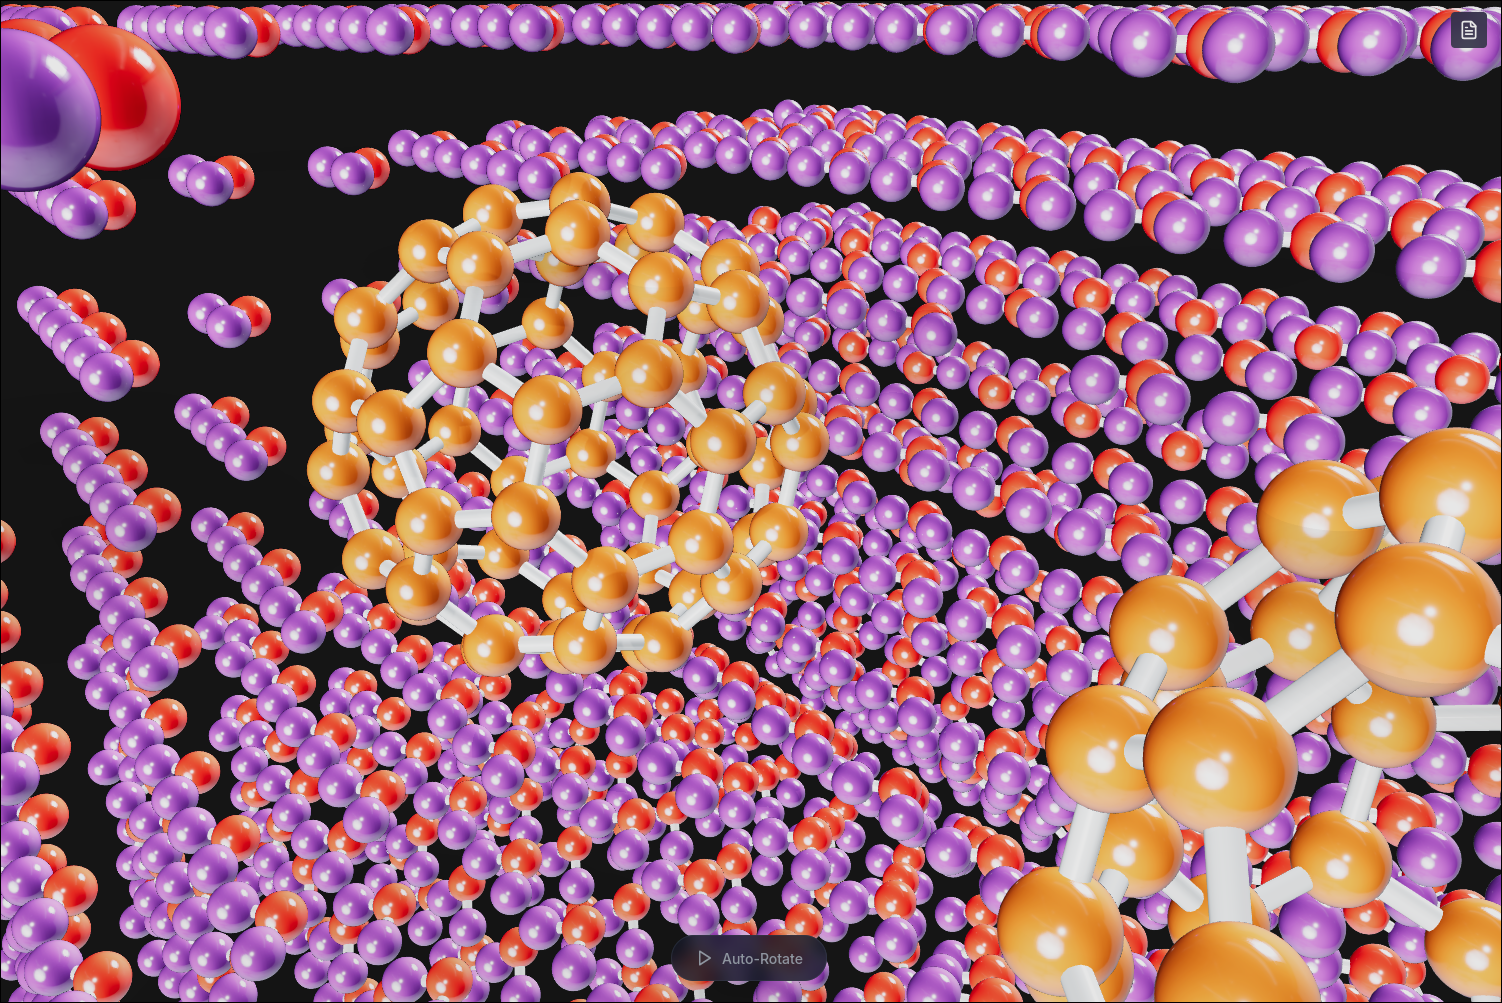
\includegraphics[width=\linewidth]{images/oplsaa_c60.png}
        \caption{\textbf{OPLS-AA}\\(Explicit Bonds / Harmonic)}
    \end{subfigure}
    \hfill
    \begin{subfigure}{0.48\textwidth}
        \centering
        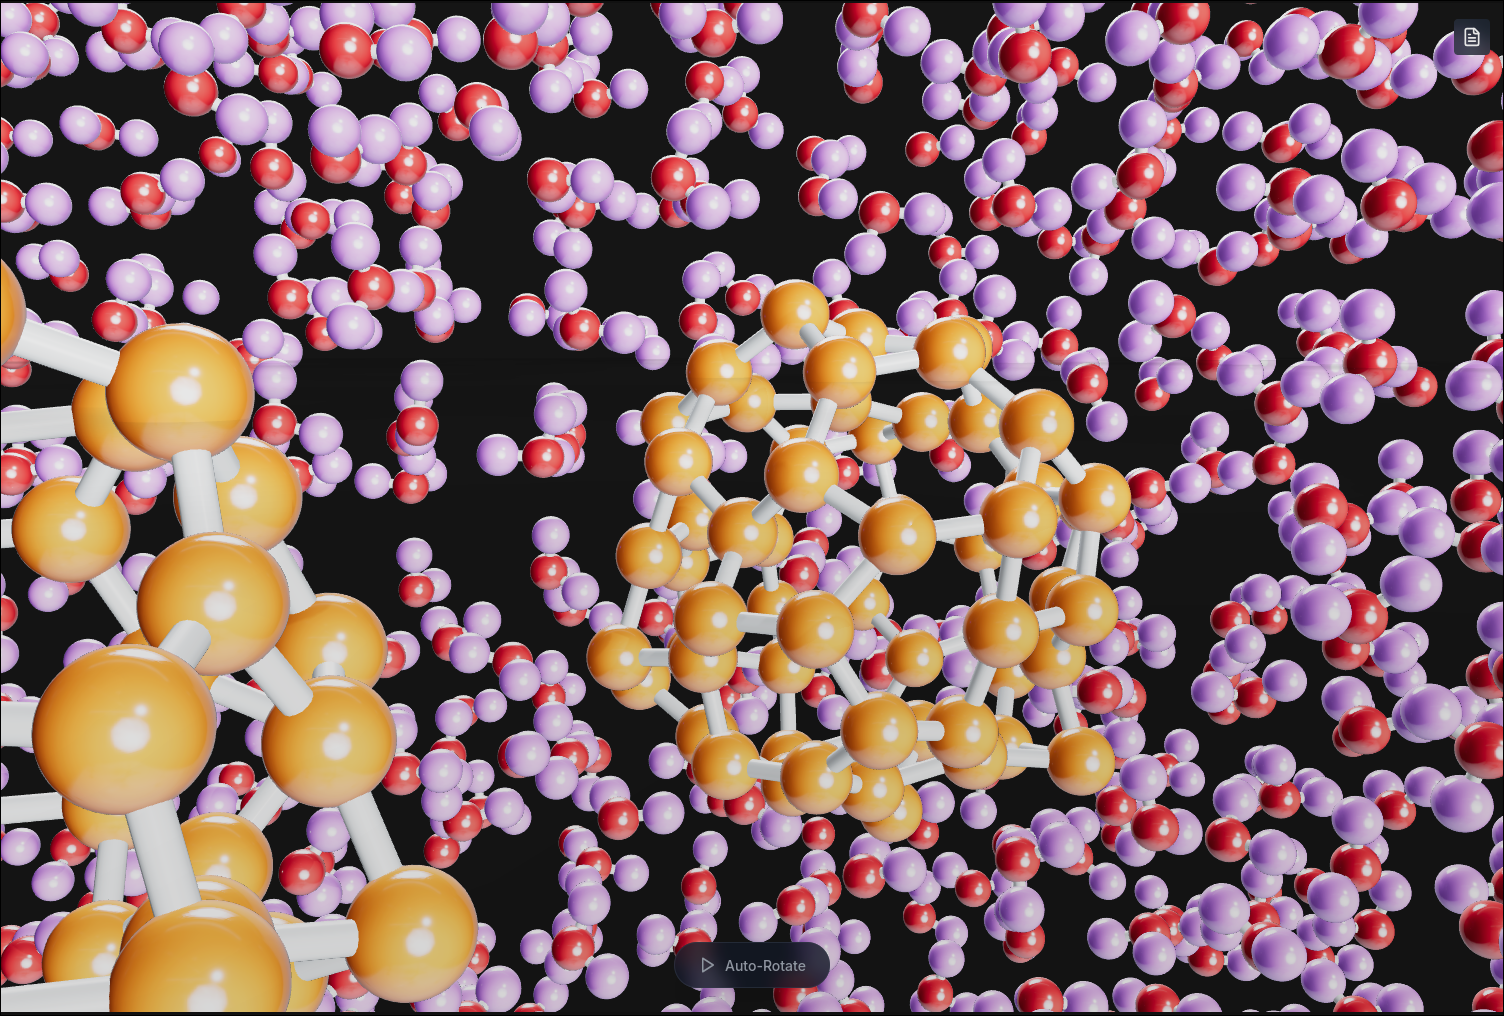
\includegraphics[width=\linewidth]{images/airebo_c60.png}
        \caption{\textbf{AIREBO}\\(Reactive / Many-Body)}
    \end{subfigure}

\end{figure}

\end{frame}


% --- SLIDE 2: Technical Explanation ---
\begin{frame}{Force Field Differences}

    % Block 1: OPLS-AA
    \begin{block}{1. OPLS-AA (Optimized Potentials for Liquid Simulations)}
        \begin{itemize}
            \item \textbf{Fixed Topology:} Connectivity is explicitly defined. Bonds cannot break.
            \item \textbf{Harmonic Potential:} Bonds are treated as springs ($K(r-r_0)^2$).
            \item \textbf{Use Case:} Best for solvent interactions where the cage is stable.
        \end{itemize}
    \end{block}

    \vspace{0.5cm}

    % Block 2: AIREBO
    \begin{block}{2. AIREBO (Adaptive Intermolecular Reactive Empirical Bond Order)}
        \begin{itemize}
            \item \textbf{Dynamic Topology:} Interactions based on local environment (no fixed bonds).
            \item \textbf{Reactive Capability:} Can simulate bond breaking and formation.
            \item \textbf{Geometry:} Naturally captures the single/double bond character of C60.
        \end{itemize}
    \end{block}

\end{frame}
\begin{frame}{Mathematical Formulation}
    \begin{columns}[T]
        
        % Column 1: OPLS-AA
        \begin{column}{0.48\textwidth}
            \begin{block}{OPLS-AA (Class I / Harmonic)}
                Based on a Taylor expansion around a fixed equilibrium ($r_0, \theta_0$).
                
                \vspace{0.5em}
                \footnotesize
                \textbf{Bond Potential:}
                $$ V_{bond} = \sum \frac{1}{2} k_b (r_{ij} - r_0)^2 $$
                
                \textbf{Non-Bonded (Lennard-Jones + Coulomb):}
                $$ V_{nb} = \sum \left[ 4\epsilon \left( \frac{\sigma}{r}^{12} - \frac{\sigma}{r}^6 \right) + \frac{q_i q_j}{4\pi\epsilon_0 r} \right] $$
            \end{block}
            \vspace{0.5em}
            \textcolor{red}{\textbf{$\times$ Fixed Topology:}} $k_b$ and $r_0$ are constants. Bonds cannot break.
        \end{column}
        
        % Column 2: AIREBO
        \begin{column}{0.48\textwidth}
            \begin{block}{AIREBO (Reactive / Many-Body)}
                Based on the Tersoff-Brenner formalism with Torsion/LJ extensions.
                
                \vspace{0.5em}
                \footnotesize
                \textbf{Interatomic Potential:}
                $$ E = \frac{1}{2} \sum_{i} \sum_{j \neq i} [V_R(r_{ij}) - \bm{b_{ij}} V_A(r_{ij})] $$
                
                \begin{itemize}
                    \item $V_R/V_A$: Pairwise Morse-like terms.
                    \item $\bm{b_{ij}}$: \textbf{Bond Order Term}. A function of local coordination ($G$) and angles ($\theta_{ijk}$).
                \end{itemize}
            \end{block}
            \vspace{0.5em}
            \textcolor{blue}{\textbf{$\checkmark$ Dynamic Topology:}} Strength depends on environment.
        \end{column}
        
    \end{columns}
\end{frame}

% --- SLIDE 2: Application to C60 Geometry ---
\begin{frame}{Application to C$_{60}$ Geometry}

    \begin{table}
        \centering
        \renewcommand{\arraystretch}{1.5}
        \begin{tabular}{p{0.45\linewidth} | p{0.45\linewidth}}
            \toprule
            \centering \textbf{OPLS-AA Approach} & \centering \textbf{AIREBO Approach} \tabularnewline
            \midrule
            Assumes Carbon is $sp^2$ planar ($\theta_0 = 120^\circ$). & Captures pyramidalization ($sp^2 \to sp^3$ character) due to curvature. \\
            
            \textbf{Single Bond Length:} Assigns generic aromatic $r_0 \approx 1.40\text{\AA}$ to all bonds. & \textbf{Dual Bond Lengths:} Naturally reproduces distinct $r_{5,6} \approx 1.45\text{\AA}$ and $r_{6,6} \approx 1.40\text{\AA}$. \\
            
            \textit{Requires:} \texttt{fix rigid} to maintain perfect $I_h$ symmetry. & \textit{Requires:} Small timestep ($0.5$ fs) to integrate high-frequency bond vibrations. \\
            \bottomrule
        \end{tabular}
    \end{table}

    \vspace{1em}
    \centering
    \textbf{Conclusion for Solvation:} Use \textbf{OPLS-AA (Rigid)} for solvent structure accuracy. Use \textbf{AIREBO} only if studying cage deformation or fracture.

\end{frame}

\begin{frame}{BTW}

\Large
\centering
Optimizing the pair coeff has results in my AIREBO C60 to be stable enough for simulation in TIP4P water. Now I do not need to \textit{freeze} it
    
\end{frame}

\begin{frame}[fragile]{Step 4: Building the Large System (\texttt{1\_build\_large\_C60\_system.lmp})}
    \textbf{Box \& Geometry:}
    \begin{lstlisting}[language=bash]
    region mybox block -20 20 -20 20 -20 20
    create_box 3 mybox ...
    \end{lstlisting}
    \textbf{Math:} Define Domain $\Omega = \{(x,y,z) | -20 \le x,y,z \le 20\}$. Volume $V = 40^3 = 64,000 \text{ \AA}^3$.

    \vspace{0.5cm}
    \textbf{Particle Placement:}
    \begin{lstlisting}[language=bash]
    read_data C60_bonded.data add append shift -8.0 0.0 0.0
    read_data C60_bonded.data add append shift 8.0 0.0 0.0
    read_data C60_bonded.data add append shift 0.0 0.0 10.0
    \end{lstlisting}
    \textbf{Math:} Affine Transformation (Translation) for molecule $k$:
    \begin{equation}
        \mathbf{r}_{i, new}^{(k)} = \mathbf{r}_{i, original} + \mathbf{T}_k \quad \text{where } \mathbf{T}_1 = \begin{bmatrix}-8\\0\\0\end{bmatrix}, \dots
    \end{equation}
\end{frame}

\begin{frame}[fragile]{Step 4: Solvation \& Smart Deletion}
    \begin{lstlisting}[language=bash]
    lattice sc 3.1
    create_atoms 0 box mol h2omol ...
    delete_atoms overlap 7.0 water_O c60_group mol yes
    \end{lstlisting}

    \textbf{Solvation Algorithm:}
    \begin{enumerate}
        \item Generate solvent grid points $P_{grid}$ via Simple Cubic (sc) lattice.
        \item Insert molecule template at each point.
    \end{enumerate}

    \textbf{Exclusion Logic (Mathematical Condition):}
    Let $S_{C60}$ be the set of all Carbon atoms. A water molecule $W$ (centered at $\mathbf{r}_O$) is deleted if:
    \begin{equation}
        \exists \mathbf{c} \in S_{C60} : ||\mathbf{r}_O - \mathbf{c}|| < R_{cutoff}
    \end{equation}
    Here, $R_{cutoff} = 7.0$ \AA. This prevents "nuclear fusion" (infinite energy overlaps) at $t=0$.
\end{frame}


\begin{frame}[fragile]{Force Field Parameters}
    \begin{lstlisting}[language=bash]
    # C60-Water Interactions (The Variable)
    pair_coeff 1 2 0.05 3.2  # C-O Interaction \footfullcite{werder2003water}
    \end{lstlisting}

    \textbf{The Study Variable $\epsilon_{CO}$:}
    The total potential energy is:
    \begin{equation}
        U_{total} = \sum_{bonds} \frac{1}{2}k_b(r-r_0)^2 + \sum_{angles} \frac{1}{2}k_\theta(\theta-\theta_0)^2 + \sum_{i<j} \left[ 4\epsilon_{ij} \left( \frac{\sigma^{12}}{r^{12}} - \frac{\sigma^6}{r^6} \right) + \frac{C q_i q_j}{r_{ij}} \right]
    \end{equation}
    
    We vary $\epsilon_{C-O}$ (1-2 interaction).
    \begin{itemize}
        \item \textbf{Low $\epsilon$:} Carbon is hydrophobic (weak attraction).
        \item \textbf{High $\epsilon$:} Carbon is hydrophilic (strong attraction).
    \end{itemize}
\end{frame}



\begin{frame}{The Physics of Epsilon ($\epsilon_{C-O}$)}

    \begin{columns}[T]
        % Left Column: Microscopic
        \begin{column}{0.48\textwidth}
            \begin{block}{1. Microscopic Potential}
                The interaction follows the Lennard-Jones 12-6 potential:
                $$ V(r) = 4\bm{\epsilon} \left[ \left(\frac{\sigma}{r}\right)^{12} - \left(\frac{\sigma}{r}\right)^{6} \right] $$
                \begin{itemize}
                    \item $\bm{\epsilon}$ is the \textbf{Depth of the Potential Well}.
                    \item $V(r_{min}) = -\bm{\epsilon}$.
                    \item It is the binding energy of a single C-O pair.
                \end{itemize}
            \end{block}
        \end{column}

        % Right Column: Macroscopic
        \begin{column}{0.48\textwidth}
            \begin{block}{2. Macroscopic Wetting}
                Linking $\epsilon$ to the Contact Angle ($\theta$) via the Young-Dupré equation and Work of Adhesion ($W_{adh}$):
                
                $$ W_{adh} \approx \int V(r) \rho dr \propto \bm{\epsilon} $$
                
                $$ \cos \theta = \frac{W_{adh}}{\gamma_{LV}} - 1 \propto \frac{\bm{\epsilon}}{\gamma_{LV}} $$
            \end{block}
        \end{column}
    \end{columns}

    \vspace{0.5cm}
    
    \begin{alertblock}{Governing Principle}
        \centering
        Local water density scales exponentially with $\epsilon$: \quad $\rho_{shell} \propto \exp(\epsilon / k_B T)$ \\
        \small Small increases in $\epsilon$ exponentially increase the probability of water occupying the solvation shell.
    \end{alertblock}

\end{frame}


\begin{frame}{Results}
\Large
\centering
\textbf{RESULTS OF MD:}
    
\end{frame}



\section{Results}
\subsection{Thermodynamics}

\begin{frame}{Temperature Stability Analysis}
    \begin{columns}[T]
        \begin{column}{0.5\textwidth}
            \begin{figure}
                \includegraphics[width=\textwidth]{images/01a_temperature_timeseries.png} % Rename your bar chart image to this
                \caption{Average Temperature vs. $\epsilon$}
            \end{figure}
        \end{column}
        \begin{column}{0.5\textwidth}
            \begin{figure}
                \includegraphics[width=\textwidth]{images/01b_temperature_summary.png} % Rename your time series image to this
                \caption{Temperature Evolution}
            \end{figure}
        \end{column}
    \end{columns}

    \vspace{0.2cm}
    \begin{alertblock}{Key Inference}
        The NVT thermostat effectively maintains the system at \textbf{299.8 $\pm$ 0.5 K} across all interaction strengths. The independence of temperature from $\epsilon$ confirms that tuning surface chemistry does not introduce artificial heating artifacts.
    \end{alertblock}
\end{frame}

% --- Section 2: Pressure ---
\subsection{Pressure}

\begin{frame}{Pressure Response and Fluctuations}
    \begin{figure}
        \centering
        \includegraphics[width=0.85\textwidth, height=0.5\textheight, keepaspectratio]{images/02_pressure_analysis.png} % Rename pressure time series
        \caption{Pressure Evolution during Production Run}
    \end{figure}
    
    \begin{itemize}
        \item \textbf{Hydrophobic ($\epsilon \approx 0$):} Higher fluctuations (0.8--1.2 atm). Caused by local density inhomogeneities (dewetting/aggregation).
        \item \textbf{Hydrophilic ($\epsilon > 0.5$):} Stabilizes closer to 1.0 atm due to uniform solvation shells.
        \item Pressure variations reflect the balance between C$_{60}$ aggregation forces and solvation forces.
    \end{itemize}
\end{frame}

% --- Section 3: Density ---
\subsection{Density}

\begin{frame}{System Density Evolution}
    \begin{figure}
        \centering
        \includegraphics[width=0.95\textwidth, height=0.55\textheight, keepaspectratio]{images/03_density_analysis.png} % Rename density composite image
    \end{figure}

    \begin{block}{Findings}
        \begin{itemize}
            \item \textbf{Global Stability:} Density remains close to bulk water ($\sim$1.0 g/cm$^3$).
            \item \textbf{Low $\epsilon$ Trend:} Slight density increase (1.00--1.02) due to C$_{60}$ aggregation creating compact clusters.
            \item \textbf{High $\epsilon$ Trend:} Slight expansion due to formation of structured hydration shells.
        \end{itemize}
    \end{block}
\end{frame}

% --- Section 4: Energy ---
\subsection{Energetics}

\begin{frame}{Potential Energy (PE) Trends}
    \begin{figure}
        \centering
        \includegraphics[width=0.98\textwidth, height=0.65\textheight, keepaspectratio]{images/04_energy_analysis.png} % Rename PE composite image
    \end{figure}

    \begin{columns}[T]
        \begin{column}{0.48\textwidth}
            \textbf{Linear Relationship:}
            $$ \Delta PE \approx -1500 \text{ kcal/mol per unit } \epsilon $$
        \end{column}
        \begin{column}{0.48\textwidth}
        \footnotesize{
            \textbf{Thermodynamic Driver:}
            Stronger C-O interactions lower the system energy, providing the driving force for dissolution over aggregation.}
        \end{column}
    \end{columns}
\end{frame}

\begin{frame}{Comparison of All}
    \begin{figure}
        \centering
        \includegraphics[width=0.8\textwidth, height=0.85\textheight, keepaspectratio]{images/05_comparison_matrix.png} % Rename KE composite image
    \end{figure}

\end{frame}

\begin{frame}{Stability Metrics Overview}
    \begin{columns}[T]
        \begin{column}{0.5\textwidth}
            \textbf{Analysis Objectives:}
            \begin{itemize}
                \item Assess statistical independence via \textbf{Effective Sample Size ($N_{eff}$)}.
                \item Quantify system stability via \textbf{Linear Drift}.
                \item Validate equilibration across all $\epsilon$ values.
            \end{itemize}
            
            \vspace{0.5cm}
            \textbf{Data Regimes:}
            \begin{itemize}
                \item $\epsilon \le 0.50$: 20,000 samples ($N_{eff} \approx 6600$).
                \item $\epsilon \ge 0.55$: 10,000 samples ($N_{eff} \approx 3300$).
            \end{itemize}
        \end{column}
        \begin{column}{0.5\textwidth}
            \begin{figure}
                \centering
                % Main summary plot showing sample sizes and drifts
                \includegraphics[width=\textwidth, height=0.7\textheight, keepaspectratio]{images/09_stability_metrics.png}
                \caption{Stability Metrics Summary}
            \end{figure}
        \end{column}
    \end{columns}
\end{frame}

% --- Slide 2: Statistical Independence ---
\begin{frame}{Statistical Independence (Autocorrelation)}
    \begin{figure}
        \centering
        \includegraphics[width=0.9\textwidth, height=0.55\textheight, keepaspectratio]{images/06_autocorrelation_analysis.png}
        \caption{Autocorrelation Functions for T, P, and $\rho$}
    \end{figure}

    \begin{block}{Observations from CSV Data}
    \footnotesize
        \begin{itemize}
            \item \textbf{Temperature ($\tau_T$):} Rapid decorrelation ($\approx 0.002$ ps). $N_{eff} \approx N_{total}/3$.
            \item \textbf{Pressure ($\tau_P$):} Similar rapid relaxation.
            \item \textbf{Density ($\tau_\rho$):} Slower relaxation ($\approx 0.05 - 0.25$ ps), indicating structural rearrangement timescales are longer than thermal fluctuations.
        \end{itemize}
    \end{block}
\end{frame}

% --- Slide 3: Convergence Traces ---
\begin{frame}{Convergence Trends (Running Averages)}
    \begin{figure}
        \centering
        \includegraphics[width=0.9\textwidth, height=0.6\textheight, keepaspectratio]{images/08_running_averages.png}
        \caption{Running Averages of Thermodynamic Properties}
    \end{figure}
    
    \footnotesize
    Running averages flatten out significantly, confirming that the system has reached a steady state suitable for production sampling.
\end{frame}

% --- Slide 4: Quantitative Drift Analysis ---
\begin{frame}{Quantitative Drift Analysis}
    \begin{table}[]
        \centering
        \resizebox{\textwidth}{!}{%
        \begin{tabular}{c | c c | c c | c c}
            \toprule
            \textbf{Epsilon} & \textbf{$\tau_\rho$ (ps)} & \textbf{$N_{eff}$ (Density)} & \textbf{Drift T} (K/ns) & \textbf{Drift P} (atm/ns) & \textbf{Drift $\rho$} (g/cm$^3$/ns) \\
            \midrule
            0.00 & 0.05 & 1777 & -0.001 & 0.083 & -3.7e-05 \\
            0.25 & 0.08 & 1794 & 0.002 & -0.083 & -1.5e-05 \\
            0.50 & 0.05 & 1775 & 0.003 & 0.052 & 9.0e-06 \\
            \textbf{0.75} & 0.06 & 910 & -0.011 & 0.402 & -4.7e-05 \\
            \textbf{1.10} & 0.08 & 807 & 0.005 & 0.008 & -2.1e-05 \\
            \bottomrule
        \end{tabular}%
        }
        \caption{Selected Metrics from \texttt{equilibration\_metrics.csv}}
    \end{table}

    \begin{alertblock}{Stability Assessment}
        \begin{itemize}
            \item \textbf{Temperature Drift:} Negligible ($< 0.01$ K/ns), indicating excellent thermostatting.
            \item \textbf{Density Drift:} Extremely low ($< 10^{-4}$ g/cm$^3$/ns), confirming structural equilibrium.
            \item \textbf{Impact of Reduced Sampling:} For $\epsilon > 0.50$, $N_{eff}$ drops but remains statistically sufficient ($>800$ independent samples).
        \end{itemize}
    \end{alertblock}
\end{frame}

% --- Slide 5: Error Estimation ---
\begin{frame}{Error Estimation (Block Averaging)}
    \begin{figure}
        \centering
        \includegraphics[width=0.85\textwidth, height=0.6\textheight, keepaspectratio]{images/07_block_averaging.png}
        \caption{Block Averaging Analysis}
    \end{figure}
    
    \centering
    Plateaus in the block averaging plots indicate that standard error estimates are reliable and internal correlations have been accounted for.
\end{frame}


\begin{frame}{Nanoparticle Aggregation (C-C Interactions)}
    \begin{figure}
        \centering
        % Place your C-C RDF comparison plot here
        \includegraphics[width=0.8\textwidth, height=0.55\textheight, keepaspectratio]{images/10_rdf_comparison.png} 
        \caption{C-C Radial Distribution Function across $\epsilon$}
    \end{figure}

    \begin{columns}[T]
        \begin{column}{0.48\textwidth}
            \textbf{Hydrophobic ($\epsilon \le 0.1$):}
            \begin{itemize}
                \item Strong contact peak at $r \approx 7-8$ \AA.
                \item Indicates direct aggregation (phase separation).
            \end{itemize}
        \end{column}
        \begin{column}{0.48\textwidth}
            \textbf{Hydrophilic ($\epsilon \ge 0.5$):}
            \begin{itemize}
                \item Contact peak vanishes.
                \item Nanoparticles are dispersed by hydration shells.
            \end{itemize}
        \end{column}
    \end{columns}
\end{frame}

% --- Slide 3: Hydration Shell Structure (C-O) ---
\begin{frame}{Hydration Shell Structure (C-O Interactions)}
    \begin{columns}[T]
        \begin{column}{0.6\textwidth}
            \begin{figure}
                \centering
                % Place your C-O RDF comparison plot here
                \includegraphics[width=\textwidth, height=0.6\textheight, keepaspectratio]{images/11_co_rdf_detailed.png}
                \caption{C-O Radial Distribution Function}
            \end{figure}
        \end{column}
        \begin{column}{0.4\textwidth}
            \textbf{Trends:}
            \begin{itemize}
                \item \textbf{Peak Height:} Increases drastically with $\epsilon$ .

            \end{itemize}
            \vspace{0.5cm}
            \textit{Interpretation:} High $\epsilon$ draws water closer, forming a dense, structured "cage" around the C$_{60}$.
        \end{column}
    \end{columns}
\end{frame}

% --- Slide 4: Detailed First Shell Analysis ---
\begin{frame}{Nano-particle-Water RDF}

            \begin{figure}
                \centering
                % Place your zoomed-in C-O plot here
                \includegraphics[width=0.9\textwidth]{images/11_co_rdf_detailed.png}
                \caption{Nano-particle-Water RDF}
            \end{figure}

    
    \vspace{0.2cm}
    \centering
    \textbf{Solvation Transition:} A sharp structural change occurs between $\epsilon=0.15$ and $0.30$.
\end{frame}

% --- Slide 5: Coordination Numbers ---
\begin{frame}{Water Coordination Number ($N_{coord}$)}
    \begin{figure}
        \centering
        % Place your bar chart of coordination numbers here
        \includegraphics[width=0.85\textwidth, height=0.75\textheight, keepaspectratio]{images/12_coordination_numbers.png}
        \caption{First Shell Coordination Number (r $<$ 5.0 \AA)}
    \end{figure}

\end{frame}

% --- Slide 6: Water Structure Perturbation (O-O) ---
\begin{frame}{Perturbation of Bulk Water (O-O Interactions)}
    \begin{figure}
        \centering
        % Place your O-O RDF plot here
        \includegraphics[width=0.9\textwidth, height=0.9\textheight, keepaspectratio]{images/10_rdf_comparison.png}
        \caption{Water-Water O-O RDF}
    \end{figure}


\end{frame}

\begin{frame}{Water Coordination and Hydrogen Bonding}
    \begin{figure}
        \centering
        \includegraphics[width=0.9\textwidth, height=0.65\textheight, keepaspectratio]{images/16_coordination_hbond_analysis.png}
        \caption{Coordination Number and H-Bond Evolution}
    \end{figure}
\end{frame}

% --- Slide 3: Coordination Trends ---
\begin{frame}{Coordination Trends: Key Findings}
    \begin{columns}[T]
        \begin{column}{0.6\textwidth}
            \textbf{1. C-C Coordination (Aggregation):}
            \begin{itemize}
                \item $\epsilon=0.0$: High ($\approx 22.4$) $\to$ Strong clustering.
                \item $\epsilon=0.15$: Drop to $\approx 19.9$ $\to$ Onset of dispersion.
                \item $\epsilon \ge 0.20$: Slight rise ($\approx 23$) likely due to dynamic re-clustering or PBC artifacts.
            \end{itemize}
            
            \vspace{0.3cm}
            \textbf{2. C-O Coordination (Solvation):}
            \begin{itemize}
                \item Monotonic increase from $5.4$ ($\epsilon=0.05$) to $11.4$ ($\epsilon=1.10$).
                \item \textbf{Interpretation:} Stronger surface attraction draws more water into the first shell, densifying the hydration layer.
            \end{itemize}
        \end{column}
        \begin{column}{0.4\textwidth}
            \begin{alertblock}{H-Bond Network}
                Total H-bonds remain stable ($\approx 2710 \pm 25$) across all $\epsilon$.
                
                \textit{Conclusion:} The gain in C-O adhesion does not catastrophically disrupt the global water network; it rearranges locally.
            \end{alertblock}
        \end{column}
    \end{columns}
\end{frame}

% --- Slide 4: Tetrahedral Order ---
\begin{frame}{Tetrahedral Order Parameter ($q$)}
    \begin{figure}
        \centering
        \includegraphics[width=0.9\textwidth, height=0.55\textheight, keepaspectratio]{images/13_tetrahedral_order_analysis.png}
        \caption{Tetrahedral Order Evolution}
    \end{figure}

    \centering
    \small
    $q \approx 0.66$ across all systems. The local tetrahedral symmetry of water is remarkably resilient, even when interacting strongly with the hydrophobic/hydrophilic surface.
\end{frame}

% --- Slide 5: Steinhardt Parameters ---
\begin{frame}{Orientational Order (Steinhardt $Q_4, Q_6$) \footfullcite{steinhardt1983bond}}
    \begin{figure}
        \centering
        \includegraphics[width=0.9\textwidth, height=0.55\textheight, keepaspectratio]{images/14_steinhardt_order_parameters.png}
        \caption{Steinhardt Order Parameters vs. $\epsilon$}
    \end{figure}
    
    \begin{itemize}
        \item \textbf{Observation:} Both $Q_4$ and $Q_6$ show a slight upward trend with $\epsilon$.
        \item \textbf{Inference:} High $\epsilon$ induces a slightly more ordered, "ice-like" structure in the hydration shell compared to the bulk-like disorder at low $\epsilon$.
    \end{itemize}
\end{frame}

% --- Slide 6: Shape Parameters ---
\begin{frame}{Cluster Shape Analysis (Asphericity \& Acylindricity)}
    \begin{figure}
        \centering
        \includegraphics[width=0.9\textwidth, height=0.55\textheight, keepaspectratio]{images/15_shape_parameters_oblate_prolate.png}
        \caption{Water Cluster Shape Anisotropy}
    \end{figure}

    \begin{itemize}
        \item \textbf{Fluctuations:} High variance in shape parameters suggests the water cluster is highly dynamic and liquid-like, not rigid.
        \item \textbf{No Phase Transition:} No sudden shape change indicates the system remains in the liquid phase throughout the transition.
    \end{itemize}
\end{frame}


\begin{frame}{Thermodynamic Response Functions}
    \begin{figure}
        \centering
        % Ensure this matches your image filename
        \includegraphics[width=0.95\textwidth, height=0.45\textheight, keepaspectratio]{images/22_thermodynamic_response_functions.png}
        \caption{Specific Heat Capacity ($C_v$) and Isothermal Compressibility ($\kappa_T$)}
    \end{figure}

\footnotesize
    \begin{columns}[T]
        \begin{column}{0.5\textwidth}
            \textbf{Specific Heat Capacity ($C_v$):}
            \begin{itemize}
                \item $C_v = \frac{\langle (\Delta E)^2 \rangle}{k_B T^2}$.
                \item Fluctuates around $\approx 0.006$ kcal/(mol$\cdot$K$\cdot$atom).
                \item \textbf{Insight:} No dramatic phase transition peak observed, suggesting the solvent remains in a single liquid phase.
            \end{itemize}
        \end{column}
        \begin{column}{0.5\textwidth}
            \textbf{Isothermal Compressibility ($\kappa_T$):}
            \begin{itemize}
                \item $\kappa_T = \frac{\langle (\Delta V)^2 \rangle}{V k_B T}$.
                \item \textbf{Low $\epsilon$:} Close to bulk water ($\approx 0.45$ GPa$^{-1}$).
                \item \textbf{High $\epsilon$:} Drops to $\approx 0.39$ GPa$^{-1}$.
                \item \textbf{Insight:} Stronger solvation shells make the system \textbf{stiffer} (less compressible) than bulk water.
            \end{itemize}
        \end{column}
    \end{columns}
\end{frame}

\begin{frame}{All the Results are in Public Domain}
    \begin{center}
        \Large \textbf{All the Results can be found at \url{https://github.com/Shuvam-Banerji-Seal/CH4114_Lammps_results_project.gi}}
    \end{center}
\end{frame}


\begin{frame}
    \centering
    \Huge \textbf{Now Comes ML Stuff!!!} \\
    \vspace{0.5cm}
    \Large All Codes are Open Sourced in my Github!!!
\end{frame}



% =========================
% ML
% =========================

\section{Executive Summary}

\begin{frame}{Executive Summary: Model Comparison}
    \begin{table}[]
        \centering
        \resizebox{\textwidth}{!}{%
        \begin{tabular}{l | c | c | c}
            \toprule
            \textbf{Feature} & \textbf{Production (Baseline)} & \textbf{Improved (Deep Physics)} & \textbf{VAE (Generative)} \\
            \midrule
            \textbf{Architecture} & MLP + LSTM & \textbf{Spectral Norm} + Residual & Probabilistic VAE \\
            \textbf{Conditioning} & Input Only & \textbf{Deep Injection (Multi-layer)} & Deep Injection \\
            \textbf{Latent Space} & Deterministic ($z$) & Deterministic ($z$) & \textbf{Stochastic ($\mu, \sigma$)} \\
            \textbf{Physics Loss} & None (Pure MSE) & \textbf{Energy + RDF Constraints} & Energy + RDF + KL \\
            \textbf{Optimizer} & AdamW & \textbf{Muon (Orthogonal)} & AdamW \\
            \textbf{Parameters} & 80.49 M & 81.51 M & 81.77 M \\
            \bottomrule
        \end{tabular}%
        }
    \end{table}

    \vspace{0.5cm}
    \textbf{Key Innovation:} The \textbf{Improved Model} introduces "Deep Conditioning" and "Physics-Informed Loss" to ensure thermodynamic consistency beyond simple data fitting.
\end{frame}

% --- Section 2: Data Flow ---
\section{Machine Learning Framework}
\subsection{Data Flow \& Training}

\begin{frame}{The "Teacher-Student" Concept}
    \begin{columns}[T]
        \begin{column}{0.5\textwidth}
            \textbf{Key Concept:} 
            The simulation data (Trajectory, Thermo, RDF) are \textbf{NOT inputs}. They are the \textbf{Ground Truth (Answers)} used to train the model.

            \vspace{0.5cm}
            \begin{itemize}
                \item \textbf{Input ($\epsilon$):} The only variable given to the model.
                \item \textbf{Model (Student):} Guesses the system state.
                \item \textbf{Loss (Teacher):} Compares the guess to the LAMMPS data.
            \end{itemize}
        \end{column}
        \begin{column}{0.5\textwidth}
            \centering
            % Placeholder for Mermaid Diagram: 7.1 Simplified Data Flow
            % [INSERT MERMAID DIAGRAM: simplified_data_flow.png]
            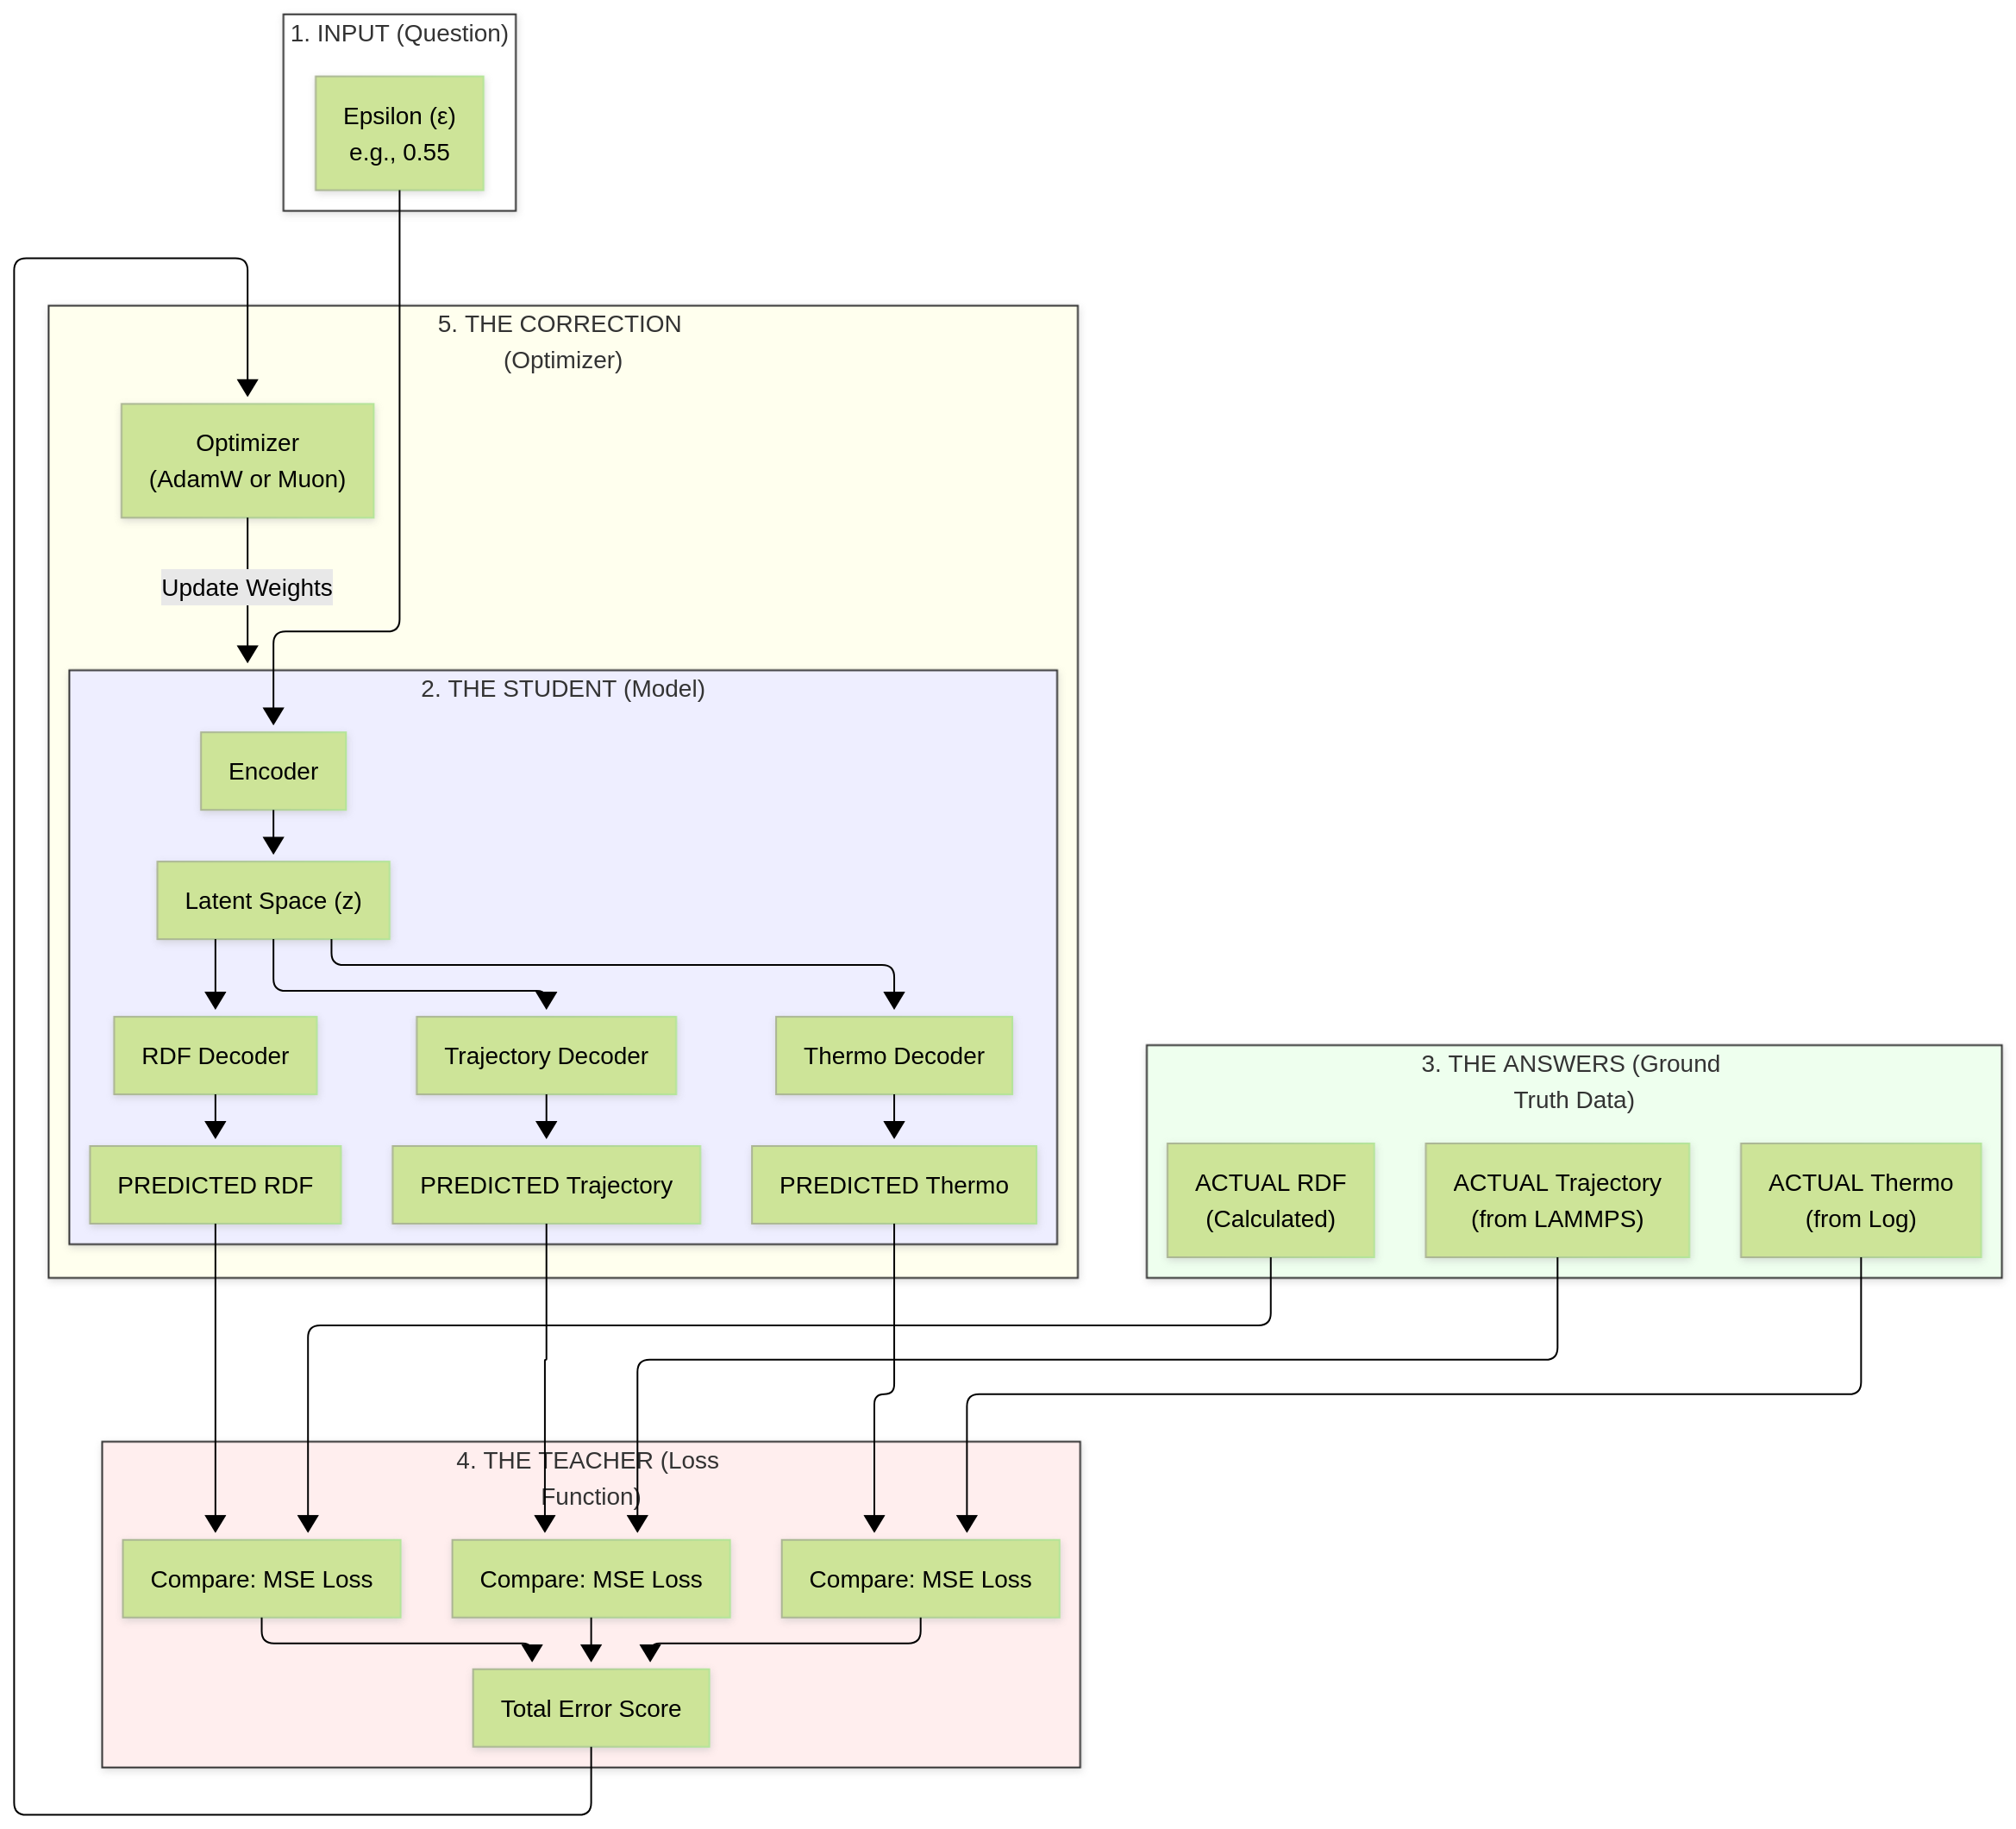
\includegraphics[width=\textwidth, height=0.7\textheight, keepaspectratio]{images/the_teacher_student_concept.png}   
        \end{column}
    \end{columns}
\end{frame}

% =================================================================
% SLIDE 1: TRAINING CONFIGURATION & INITIALIZATION
% =================================================================
\begin{frame}[fragile]{Training Strategy: Improved Model (Part 1)}
    \centering
    \footnotesize
    \begin{algorithm}[H]
        \caption*{Physics-Informed Training Loop (Initialization)}
        \footnotesize
        \begin{algorithmic}[1]
            \footnotesize
            \Require $\mathcal{D}_{train} = \{(\epsilon_i, X_i, S_i, g(r)_i)\}$, Epochs $E$, Batch $B$
            
            \State \textbf{Initialize Model:} $\mathcal{M}_{\theta}$ (Improved Architecture)
            \State \textbf{Optimizer:} 
            \If{\texttt{has\_muon}}
                \State $\text{Opt} \leftarrow \text{Muon}(\theta, \text{lr}=5\text{e-}5, \text{momentum}=0.9)$ \footfullcite{jordan2024muon}
            \Else
                \State $\text{Opt} \leftarrow \text{AdamW}(\theta, \text{lr}=5\text{e-}5, \text{wd}=1\text{e-}4)$ \footfullcite{loshchilov2017decoupled}
            \EndIf
            
            \State \textbf{Scheduler:} CosineAnnealingLR($T_{max}=E, \eta_{min}=1\text{e-}6$) \footfullcite{loshchilov2016sgdr}
            \State \textbf{Scaler:} GradScaler (for Mixed Precision FP16)
            \State \textbf{Loss weights:} $\alpha_{\text{traj}}=1, \alpha_{\text{thermo}}=2, \alpha_{\text{rdf}}=5, \alpha_{\text{phys}}=0.5$
            
            \Statex \hrulefill
            \algstore{train_algo}
        \end{algorithmic}
    \end{algorithm}
\end{frame}

% =================================================================
% SLIDE 2: THE TRAINING LOOP (FORWARD PASS)
% =================================================================
\begin{frame}[fragile]{Training Strategy: Forward Pass \& Physics Loss}
    \centering
    \begin{algorithm}[H]
        \caption*{Physics-Informed Training Loop (Forward)}
        \begin{algorithmic}[1]
            \algrestore{train_algo}
            
            \For{$\text{epoch} = 1 \to E$}
                \State $\mathcal{M}_{\theta}.\text{train}()$
                \For{$\text{batch} (\epsilon, \mathbf{y}_{true}) \in \mathcal{D}_{train}$}
                    
                    \LineComment{Forward Pass with Mixed Precision}
                    \State $\mathbf{y}_{pred} \leftarrow \mathcal{M}_{\theta}(\epsilon)$
                    
                    \LineComment{Compute Component Losses}
                    \State $\mathcal{L}_{MSE} \leftarrow \text{MSE}(\mathbf{y}_{pred}, \mathbf{y}_{true})$
                    \State $\mathcal{L}_{phys} \leftarrow \text{PhysicsLoss}(\mathbf{y}_{pred}, \epsilon)$
                    \State \hspace{2em} \textit{(Energy Conservation + Thermodynamic Consistency)}
                    
                    \LineComment{Total Weighted Loss}
                    \State $\mathcal{L}_{total} \leftarrow \alpha \cdot \mathcal{L}_{MSE} + \alpha_{phys} \cdot \mathcal{L}_{phys}$
                    
                    \If{\text{use\_vae}}
                        \State $\mathcal{L}_{total} \leftarrow \mathcal{L}_{total} + \beta \cdot D_{KL}(q(z|x) || \mathcal{N}(0,I))$
                    \EndIf
                    
                    \algstore{train_algo_2}
        \end{algorithmic}
    \end{algorithm}
\end{frame}

% =================================================================
% SLIDE 3: BACKPROP & OPTIMIZATION
% =================================================================
\begin{frame}[fragile]{Training Strategy: Optimization \& Monitoring}
    \centering
    \begin{algorithm}[H]
        \caption*{Physics-Informed Training Loop (Optimization)}
        \begin{algorithmic}[1]
            \algrestore{train_algo_2}
            
                    \LineComment{Backward Pass with Gradient Accumulation}
                    \State $\text{Scaler}.\text{scale}(\mathcal{L}_{total})$.backward()
                    
                    \If{$\text{step} \% \text{accum\_steps} == 0$}
                        \State $\text{ClipGradients}(\theta, \text{max\_norm}=1.0)$
                        \State $\text{Scaler}.\text{step}(\text{Opt})$
                        \State $\text{Scaler}.\text{update}()$
                        \State $\text{Opt}.\text{zero\_grad}()$
                    \EndIf
                \EndFor
                
                \LineComment{End of Epoch}
                \State $\text{Scheduler}.\text{step}()$
                \State \textbf{Validate:} Compute $\mathcal{L}_{val}$ on unseen $\epsilon$
                
                \If{$\mathcal{L}_{val} < \mathcal{L}_{best}$}
                    \State $\mathcal{L}_{best} \leftarrow \mathcal{L}_{val}$
                    \State \textbf{Save Checkpoint:} \texttt{best\_model.pt}
                \EndIf
                
                \If{$\text{epoch} \% 10 == 0$}
                    \State \textbf{Analyze Latent:} t-SNE / PCA of $z$ space
                \EndIf
                
            \EndFor
        \end{algorithmic}
    \end{algorithm}
\end{frame}

\begin{frame}[fragile]{Model Architecture: Input \& Encoder}
    \centering
    \begin{algorithm}[H]
        \caption*{End-to-End Pipeline Overview (Part 1)}
        \begin{algorithmic}[1]
            % Input Stage
            \State \textbf{Input Stage}
            \State \hspace{1em} Lennard-Jones parameter $\varepsilon \in [0,0.5]$
            
            \Statex \hrulefill
            
            % Encoder Network
            \State \textbf{Encoder Network}
            \State \hspace{1em} $\varepsilon \rightarrow \text{Linear}(1,128) + \text{SpectralNorm}$
            \State \hspace{2em} $\rightarrow \text{BatchNorm1d}(128) \rightarrow \text{ReLU} \rightarrow \text{Dropout}(0.15/0.20)$
            
            \vspace{0.2em}
            \State \hspace{1em} $\rightarrow \text{Linear}(128,256) + \text{SpectralNorm}$
            \State \hspace{2em} $\rightarrow \text{BatchNorm1d}(256) \rightarrow \text{ReLU} \rightarrow \text{Dropout}(0.15/0.20)$
            
            \vspace{0.2em}
            \State \hspace{1em} $\rightarrow \text{Linear}(256,512) + \text{SpectralNorm}$
            \State \hspace{2em} $\rightarrow \text{BatchNorm1d}(512) \rightarrow \text{ReLU} \rightarrow \text{Dropout}(0.10)$
            
            \State \hspace{1em} $\rightarrow$ \textbf{Latent Projection}
            
            % Store the state of the algorithm to resume on next slide
            \algstore{myalg}
        \end{algorithmic}
    \end{algorithm}
\end{frame}

\begin{frame}{The Parameter Count}
\begin{figure}
    \centering
    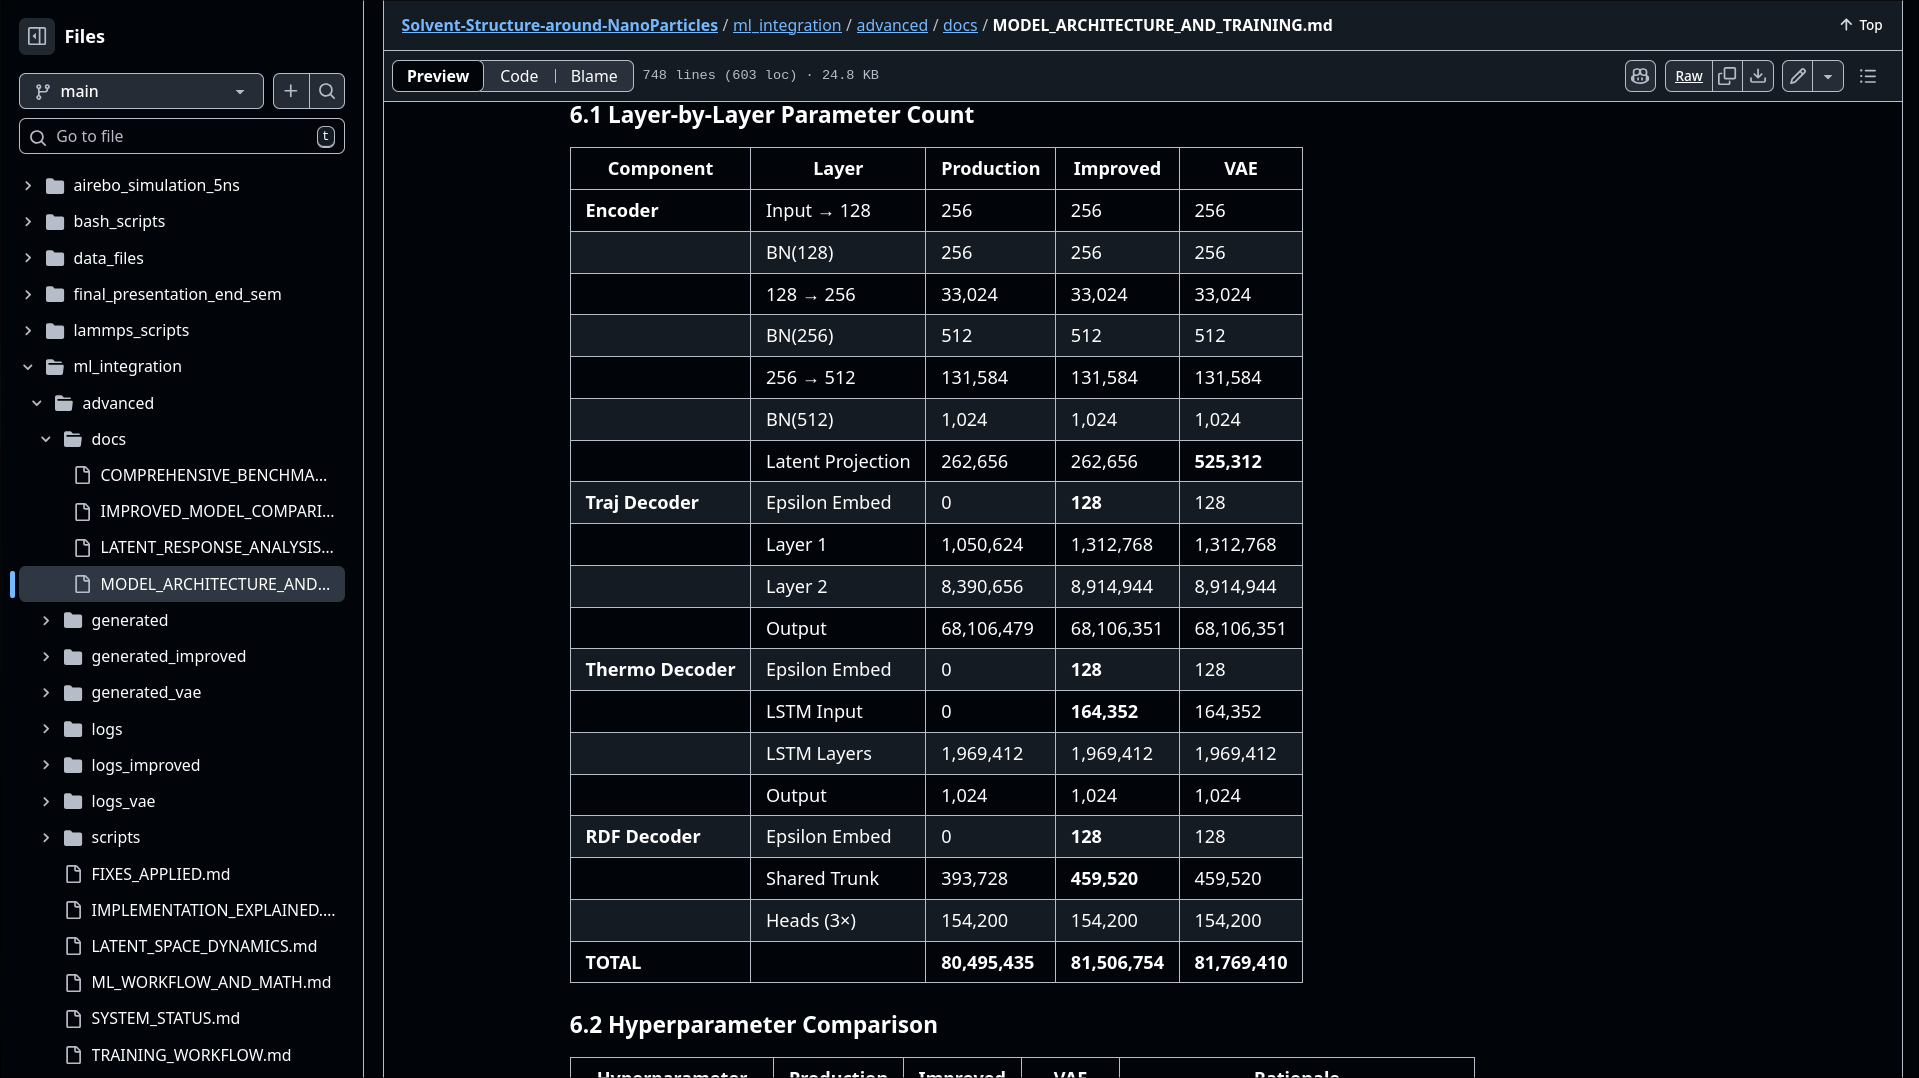
\includegraphics[width=0.8\linewidth]{images/parameter_count.png}
    \caption{The detailed explaination of the ML architecture can be found on my Github}
    \label{fig:placeholder}
\end{figure}    
\end{frame}

% =================================================================
% SLIDE 2: LATENT SPACE AND CONDITIONING
% =================================================================
\begin{frame}[fragile]{Model Architecture: Latent Space \& Conditioning}
    \centering
    \begin{algorithm}[H]
        \caption*{End-to-End Pipeline Overview (Part 2)}
        \begin{algorithmic}[1]
            % Restore the state (line numbers continue)
            \algrestore{myalg}
            
            % Latent Representations
            \State \textbf{Latent Representations}
            \State \hspace{1em} \textit{Deterministic AE:} $z_{\mathrm{det}} \in \mathbb{R}^{512}$
            \State \hspace{1em} \textit{VAE:} $\mu, \log\sigma^2 \in \mathbb{R}^{512}$
            \State \hspace{1em} \textbf{Reparameterization:}
            \[
                z_{\mathrm{vae}} = \mu + \sigma \cdot \epsilon, \qquad \epsilon \sim \mathcal{N}(0,I)
            \]
            
            \Statex \hrulefill
            
            % Epsilon Conditioning
            \State \textbf{Epsilon Conditioning (Improved Model)}
            \State \hspace{1em} $\varepsilon \rightarrow \text{Linear}(1,128) \rightarrow \text{embedding } e \in \mathbb{R}^{128}$
            \State \hspace{1em} $e$ is injected into all decoder branches.
            
            % Store again for the final slide
            \algstore{myalg}
        \end{algorithmic}
    \end{algorithm}
\end{frame}

% =================================================================
% SLIDE 3: DECODERS AND OUTPUT
% =================================================================
\begin{frame}[fragile]{Model Architecture: Decoders \& Output}
    \centering
    \begin{algorithm}[H]
        \caption*{End-to-End Pipeline Overview (Part 3)}
        \begin{algorithmic}[1]
            \algrestore{myalg}
            
            % Decoder Networks
            \State \textbf{Decoder Networks} (Inputs: $z_{\mathrm{det/vae}} \oplus e$)
            
            \vspace{0.3em}
            \State \hspace{1em} \textbf{Trajectory Decoder:}
            \State \hspace{2em} $\rightarrow X \in \mathbb{R}^{5541 \times 3}$
            
            \vspace{0.3em}
            \State \hspace{1em} \textbf{Thermodynamics Decoder:}
            \State \hspace{2em} $\rightarrow S \in \mathbb{R}^{L \times 4} \quad (T, P, \rho, PE)$
            
            \vspace{0.3em}
            \State \hspace{1em} \textbf{RDF Decoder:}
            \State \hspace{2em} $\rightarrow [g_{CC}, g_{CO}, g_{OO}] \in \mathbb{R}^{200}$
            
            \Statex \hrulefill
            
            % Final Outputs
            \State \textbf{Final Outputs}
            \[
                X \text{ (Coords)}, \quad S \text{ (Thermo)}, \quad g(r) \text{ (Structure)}
            \]
        \end{algorithmic}
    \end{algorithm}
\end{frame}
    

% --- Section 3: Architectures ---
\subsection{Detailed Architecture}

\begin{frame}{Trajectory Decoder: Production vs. Improved}
    \begin{columns}[T]
        \begin{column}{0.48\textwidth}
            \textbf{Production (Standard MLP)}
            \begin{itemize}
                \item Simple feed-forward network.
                \item $\epsilon$ is only seen at the very beginning.
                \item Risk: Model "forgets" $\epsilon$ in deep layers.
            \end{itemize}
            $$ h_l = \text{ReLU}(W_l h_{l-1} + b_l) $$
        \end{column}
        \begin{column}{0.48\textwidth}
            \textbf{Improved (Deep Conditioning)}
            \begin{itemize}
                \item $\epsilon$ is embedded ($e$) and \textbf{re-injected} at every layer.
                \item Ensures interaction strength guides every transformation step.
            \end{itemize}
            $$ h_l = \text{ReLU}(W_l [h_{l-1} \oplus e] + b_l) $$
        \end{column}
    \end{columns}

    \vspace{0.5cm}
    \centering
    % Placeholder for Mermaid Diagram: 2.2 Trajectory Decoder
    % [INSERT MERMAID DIAGRAM: trajectory_decoder.png]
    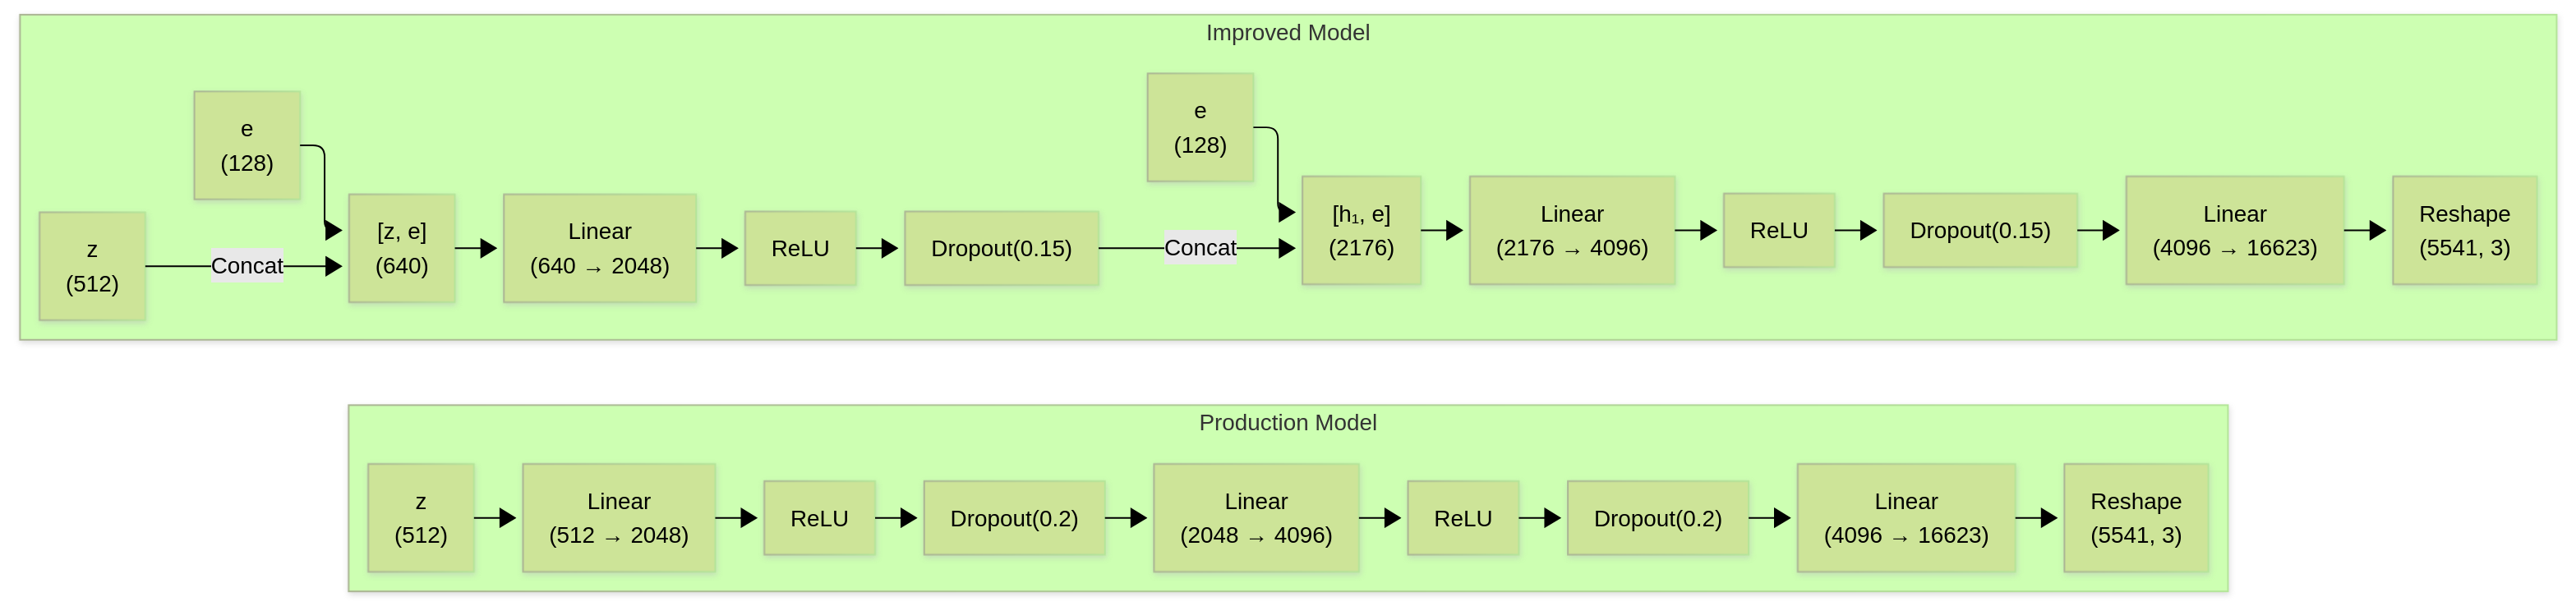
\includegraphics[width=0.8\textwidth, height=0.4\textheight, keepaspectratio]{images/trajectory_decoder.png}
\end{frame}

\begin{frame}{Thermodynamics Decoder (LSTM)}
    \textbf{Objective:} Predict time-series properties ($T, P, \rho, PE$).
    
    \vspace{0.3cm}
    \begin{columns}[T]
        \begin{column}{0.6\textwidth}
            \textbf{Architecture:}
            \begin{itemize}
                \item 3-Layer LSTM (Long Short-Term Memory).
                \item Input: Latent vector $z$ (repeated for $L$ timesteps).
                \item \textbf{Why LSTM?} Captures temporal correlations and fluctuations inherent in MD simulations.
            \end{itemize}
        \end{column}
        \begin{column}{0.4\textwidth}
            % Placeholder for Mermaid Diagram: 2.3 LSTM Decoder
            % [INSERT MERMAID DIAGRAM: lstm_decoder.png]
            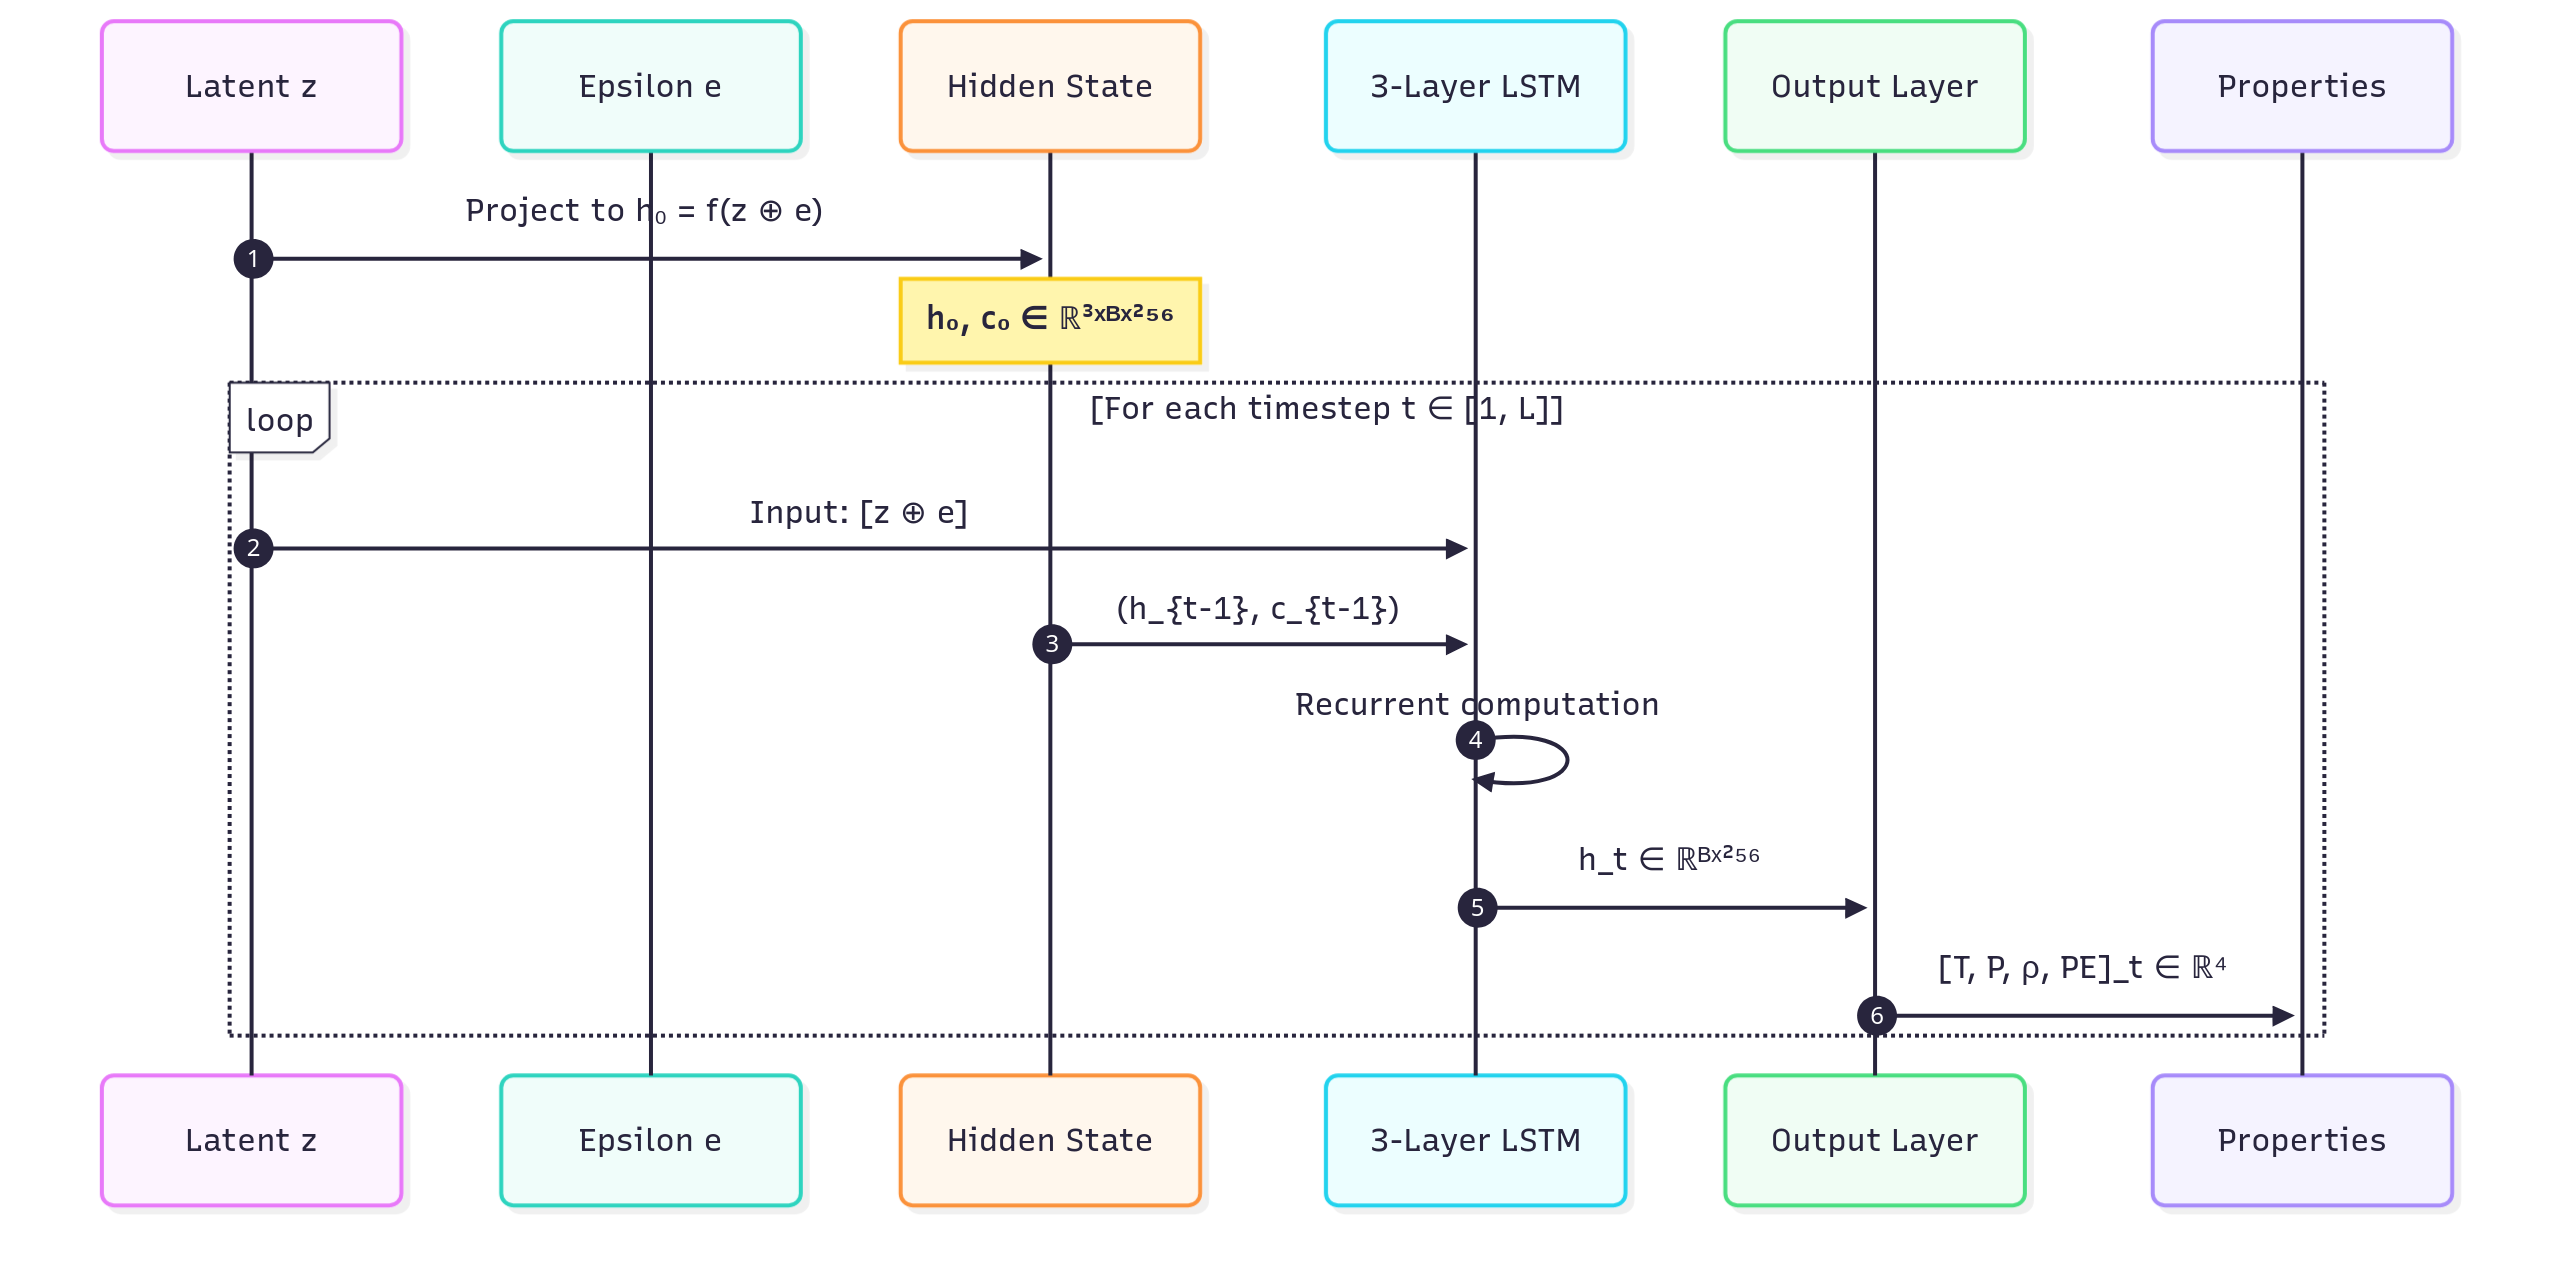
\includegraphics[width=\textwidth, height=0.8\textheight, keepaspectratio]{images/lstm_thermodynamics_decoder.png}  
        \end{column}
    \end{columns}
\end{frame}

\begin{frame}{RDF Decoder: Structure Prediction}
    \textbf{Objective:} Predict Radial Distribution Functions ($g_{CC}, g_{CO}, g_{OO}$).
    
    \vspace{0.3cm}
    \begin{columns}[T]
        \begin{column}{0.5\textwidth}
            \textbf{Design Choices:}
            \begin{itemize}
                \item \textbf{Shared Trunk:} Extracts common structural features.
                \item \textbf{Multi-Head Output:} Separate heads for C-C, C-O, and O-O correlations.
                \item \textbf{Softplus Activation:} $f(x) = \ln(1 + e^x)$.
                \begin{itemize}
                    \item Ensures $g(r) \ge 0$ (Probability cannot be negative).
                    \item Smooth gradients for training stability.
                \end{itemize}
            \end{itemize}
        \end{column}
        \begin{column}{0.5\textwidth}
            % Placeholder for Mermaid Diagram: 2.4 RDF Decoder
            % [INSERT MERMAID DIAGRAM: rdf_decoder.png]
            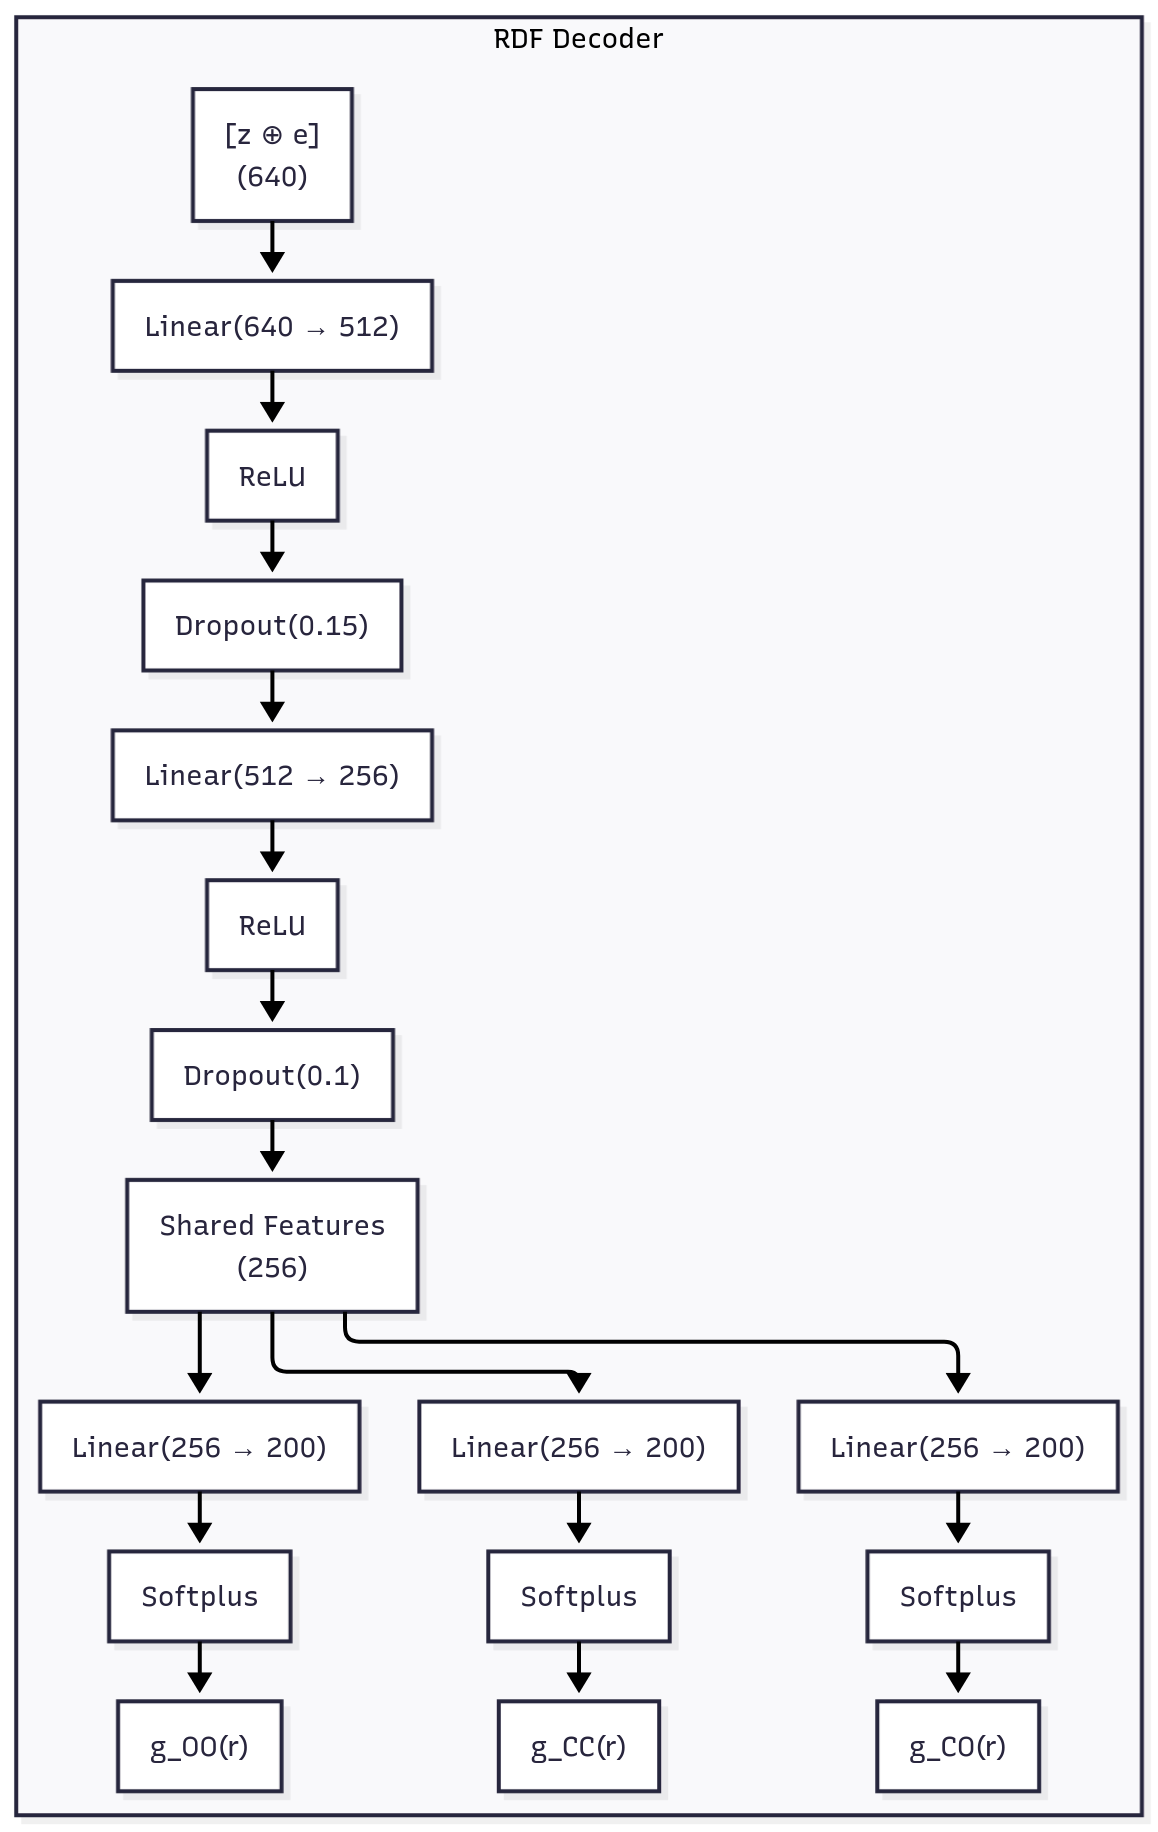
\includegraphics[width=\textwidth, height=0.8\textheight, keepaspectratio]{images/rdf_decoder.png}
        \end{column}
    \end{columns}
\end{frame}

% --- Section 4: Physics Integration ---
\subsection{Physics Integration}

\begin{frame}{Physics-Informed Loss Function}
    The "Physics Knowledge" is embedded in the Loss Function, acting as a regularizer.
    
    $$ \mathcal{L}_{total} = \mathcal{L}_{MSE} + \alpha_{phys}\mathcal{L}_{physics} $$

    \begin{block}{Physical Constraints ($\mathcal{L}_{physics}$)}
        \begin{enumerate}
            \item \textbf{Energy Conservation:} In NVT, Total Energy ($E_{tot} = PE + KE$) should be conserved.
            $$ \mathcal{L}_{energy} = \text{std}(PE + KE) $$
            \item \textbf{Thermodynamic Consistency:} Temperature is defined by Kinetic Energy.
            $$ KE_{pred} \approx \frac{3}{2} N k_B T_{pred} $$
            \item \textbf{Structural Validity:} RDFs must be non-negative.
            $$ \mathcal{L}_{RDF} = \text{ReLU}(-g(r)) $$
        \end{enumerate}
    \end{block}
\end{frame}

\begin{frame}{VAE Regularization (KL Divergence)}
\footnotesize
    For the VAE model, we enforce a structured latent space using the **Kullback-Leibler (KL) Divergence**.

    $$ \mathcal{L}_{KL} = -\frac{1}{2} \sum \left(1 + \log(\sigma^2) - \mu^2 - \sigma^2\right) $$

    \begin{columns}[T]
        \begin{column}{0.5\textwidth}
            \textbf{Effect:}
            \begin{itemize}
                \item Forces latent distribution $q(z|\epsilon)$ to approximate a standard normal $\mathcal{N}(0,I)$.
                \item Ensures smooth interpolation between $\epsilon$ values.
            \end{itemize}
        \end{column}
        \begin{column}{0.5\textwidth}
            \textbf{Reparameterization Trick:}
            Allows backpropagation through random sampling:
            $$ z = \mu + \sigma \odot \eta, \quad \eta \sim \mathcal{N}(0,I) $$
        \end{column}
    \end{columns}
\end{frame}

% --- Section 5: Optimization ---
\subsection{Optimization}

\begin{frame}{Optimizer: AdamW vs. Muon}
    The \textbf{Improved Model} utilizes the state-of-the-art \textbf{\textit{Muon}} optimizer \footfullcite{jordan2024muon}.

    \begin{table}[]
        \centering
        \begin{tabular}{l | p{5cm} | p{5cm}}
            \toprule
            & \textbf{AdamW} (Standard) & \textbf{Muon} (Advanced) \\
            \midrule
            \textbf{Logic} & Scales updates by gradient variance ("Adaptive Moment Estimation"). & Momentum \textbf{Orthogonal} Optimizer. \\
            \textbf{Math} & $w \leftarrow w - \eta \frac{\hat{m}}{\sqrt{\hat{v}} + \epsilon}$ & Uses Newton-Schulz iteration to orthogonalize updates. \\
            \textbf{Benefit} & Reliable baseline. & Better generalization for large generative models. \\
            \bottomrule
        \end{tabular}
    \end{table}
    
    \centering
    % Placeholder for Mermaid Diagram: 7.4 Optimizer Comparison
    % [INSERT MERMAID DIAGRAM: optimizer_comparison.png]
    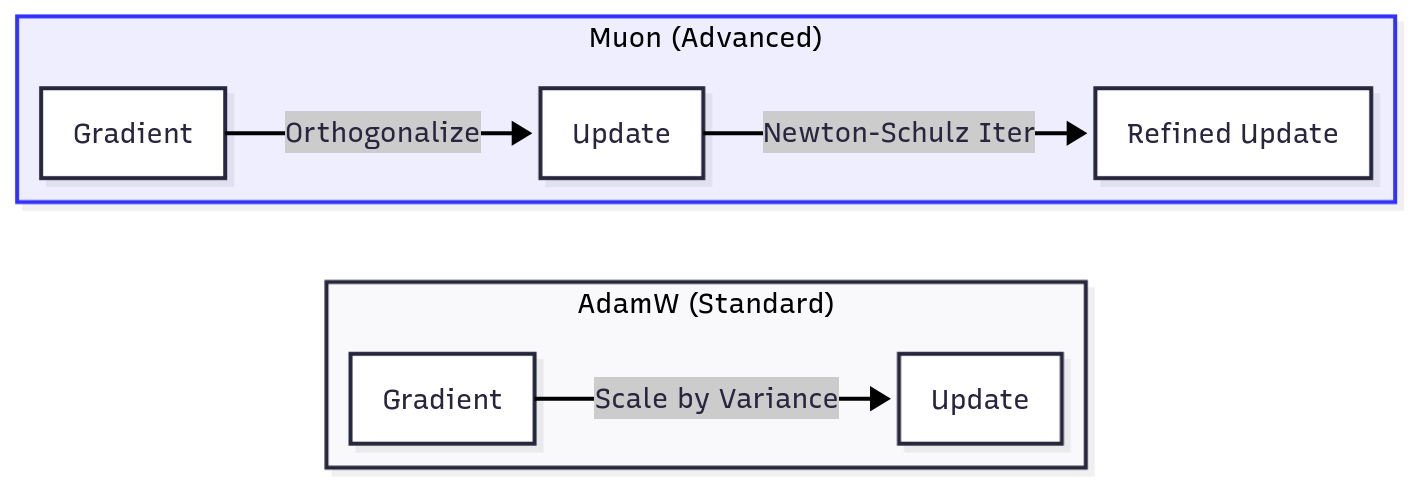
\includegraphics[width=0.6\textwidth, height=0.4\textheight, keepaspectratio]{images/optimizer_adamw_vs_muon.png}
\end{frame}

\begin{frame}{Training Workflow}
    \begin{figure}
        \centering
        % Placeholder for Mermaid Diagram: 3.1 Training Loop
        % [INSERT MERMAID DIAGRAM: training_loop.png]
        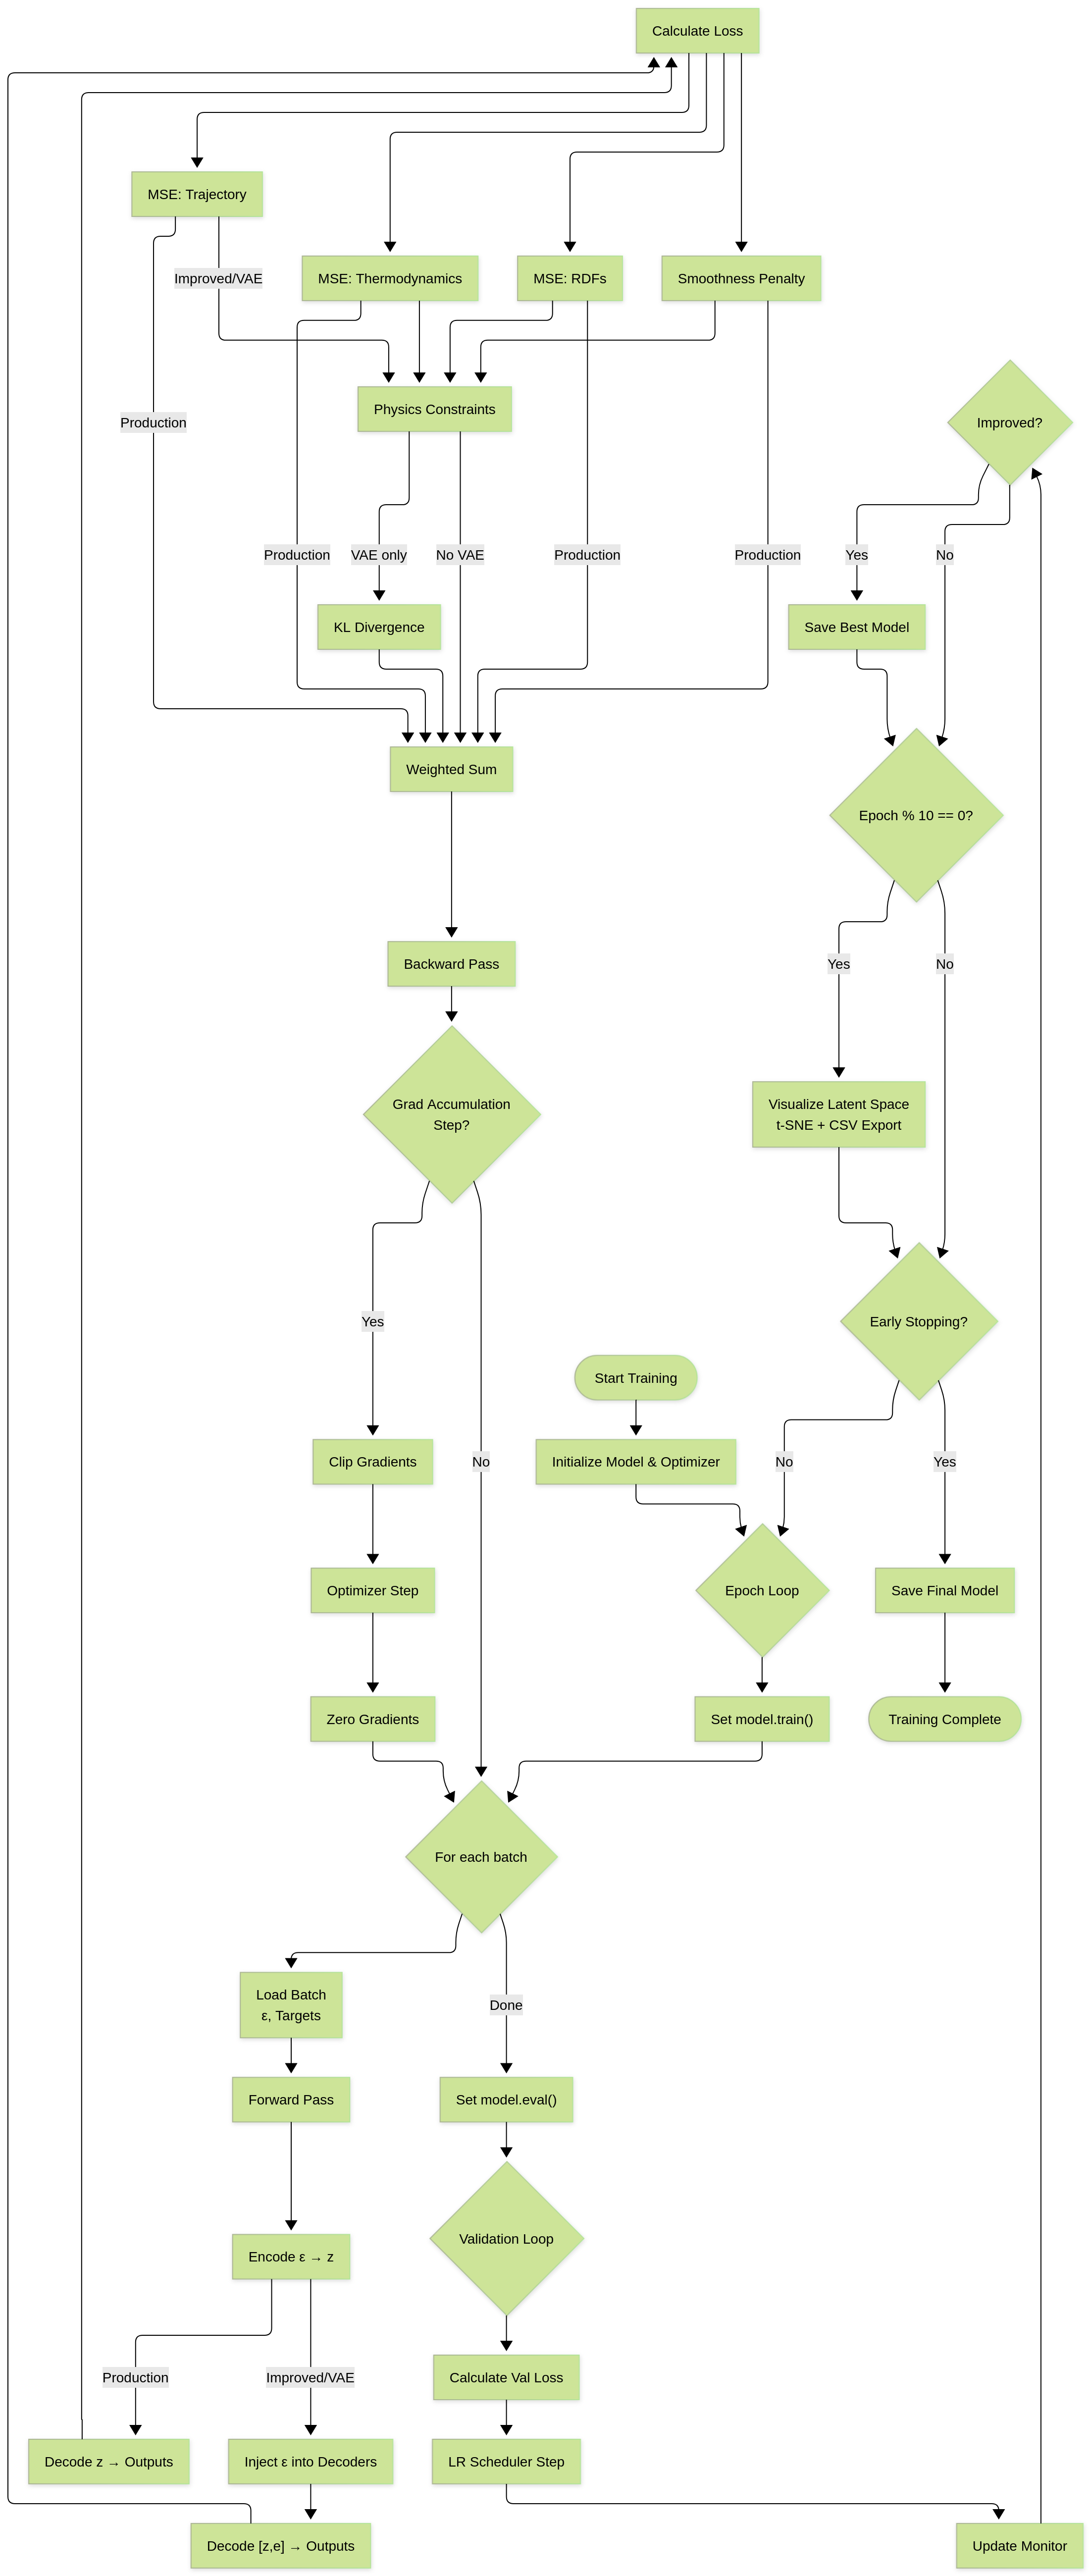
\includegraphics[width=0.9\textwidth, height=0.75\textheight, keepaspectratio]{images/complete_model_training.png}
        \caption{Complete Training Cycle with Gradient Accumulation}
    \end{figure}
\end{frame}

% --- Conclusion ---
\section{Conclusion}

\begin{frame}{Summary of ML Integration}
    \begin{enumerate}
        \item \textbf{Architecture:} Moved from simple MLP (Production) to \textbf{Deeply Conditioned Residual Networks} (Improved).
        \item \textbf{Physics Awareness:} Integrated fundamental laws (Energy Conservation, RDF constraints) directly into the loss function.
        \item \textbf{Optimization:} Adopted \textbf{Muon} optimizer for orthogonal weight updates, ensuring robust convergence in high-dimensional latent spaces.
        \item \textbf{Generative Capability:} VAE model enables probabilistic sampling of new system states, not just interpolation.
    \end{enumerate}

    \vspace{0.5cm}
    \centering
    \textbf{Result:} A model that doesn't just "memorize" data, but "understands" the underlying physics of solvation.
\end{frame}



\begin{frame}{Results of the ML model}
\centering
\Huge
\textbf{Let's see how well the model predicts!!!}
    
\end{frame}


\begin{frame}{Executive Summary: State-of-the-Art Performance}
    \begin{columns}[T]
        \begin{column}{0.5\textwidth}
            \begin{block}{Model Architecture}
                \begin{itemize}
                    \item \textbf{Parameters:} 81.51 M (+1.26\%)
                    \item \textbf{Latency:} $\sim$25s / epoch (-44\%)
                    \item \textbf{Key Tech:} Spectral Norm + Deep Conditioning
                \end{itemize}
            \end{block}
            
            \vspace{0.5cm}
            \textbf{Performance Highlights:}
            \begin{itemize}
                \item \textbf{Latent Linearity:} \textbf{97.55\%} (Correlation with $\epsilon$)
                \item \textbf{Temp Accuracy:} RMSE $\approx$ 2.4 K
                \item \textbf{Structure:} C-C RDF Correlation $>$ 0.70
            \end{itemize}
        \end{column}
        \begin{column}{0.5\textwidth}
            \begin{figure}
                \centering
                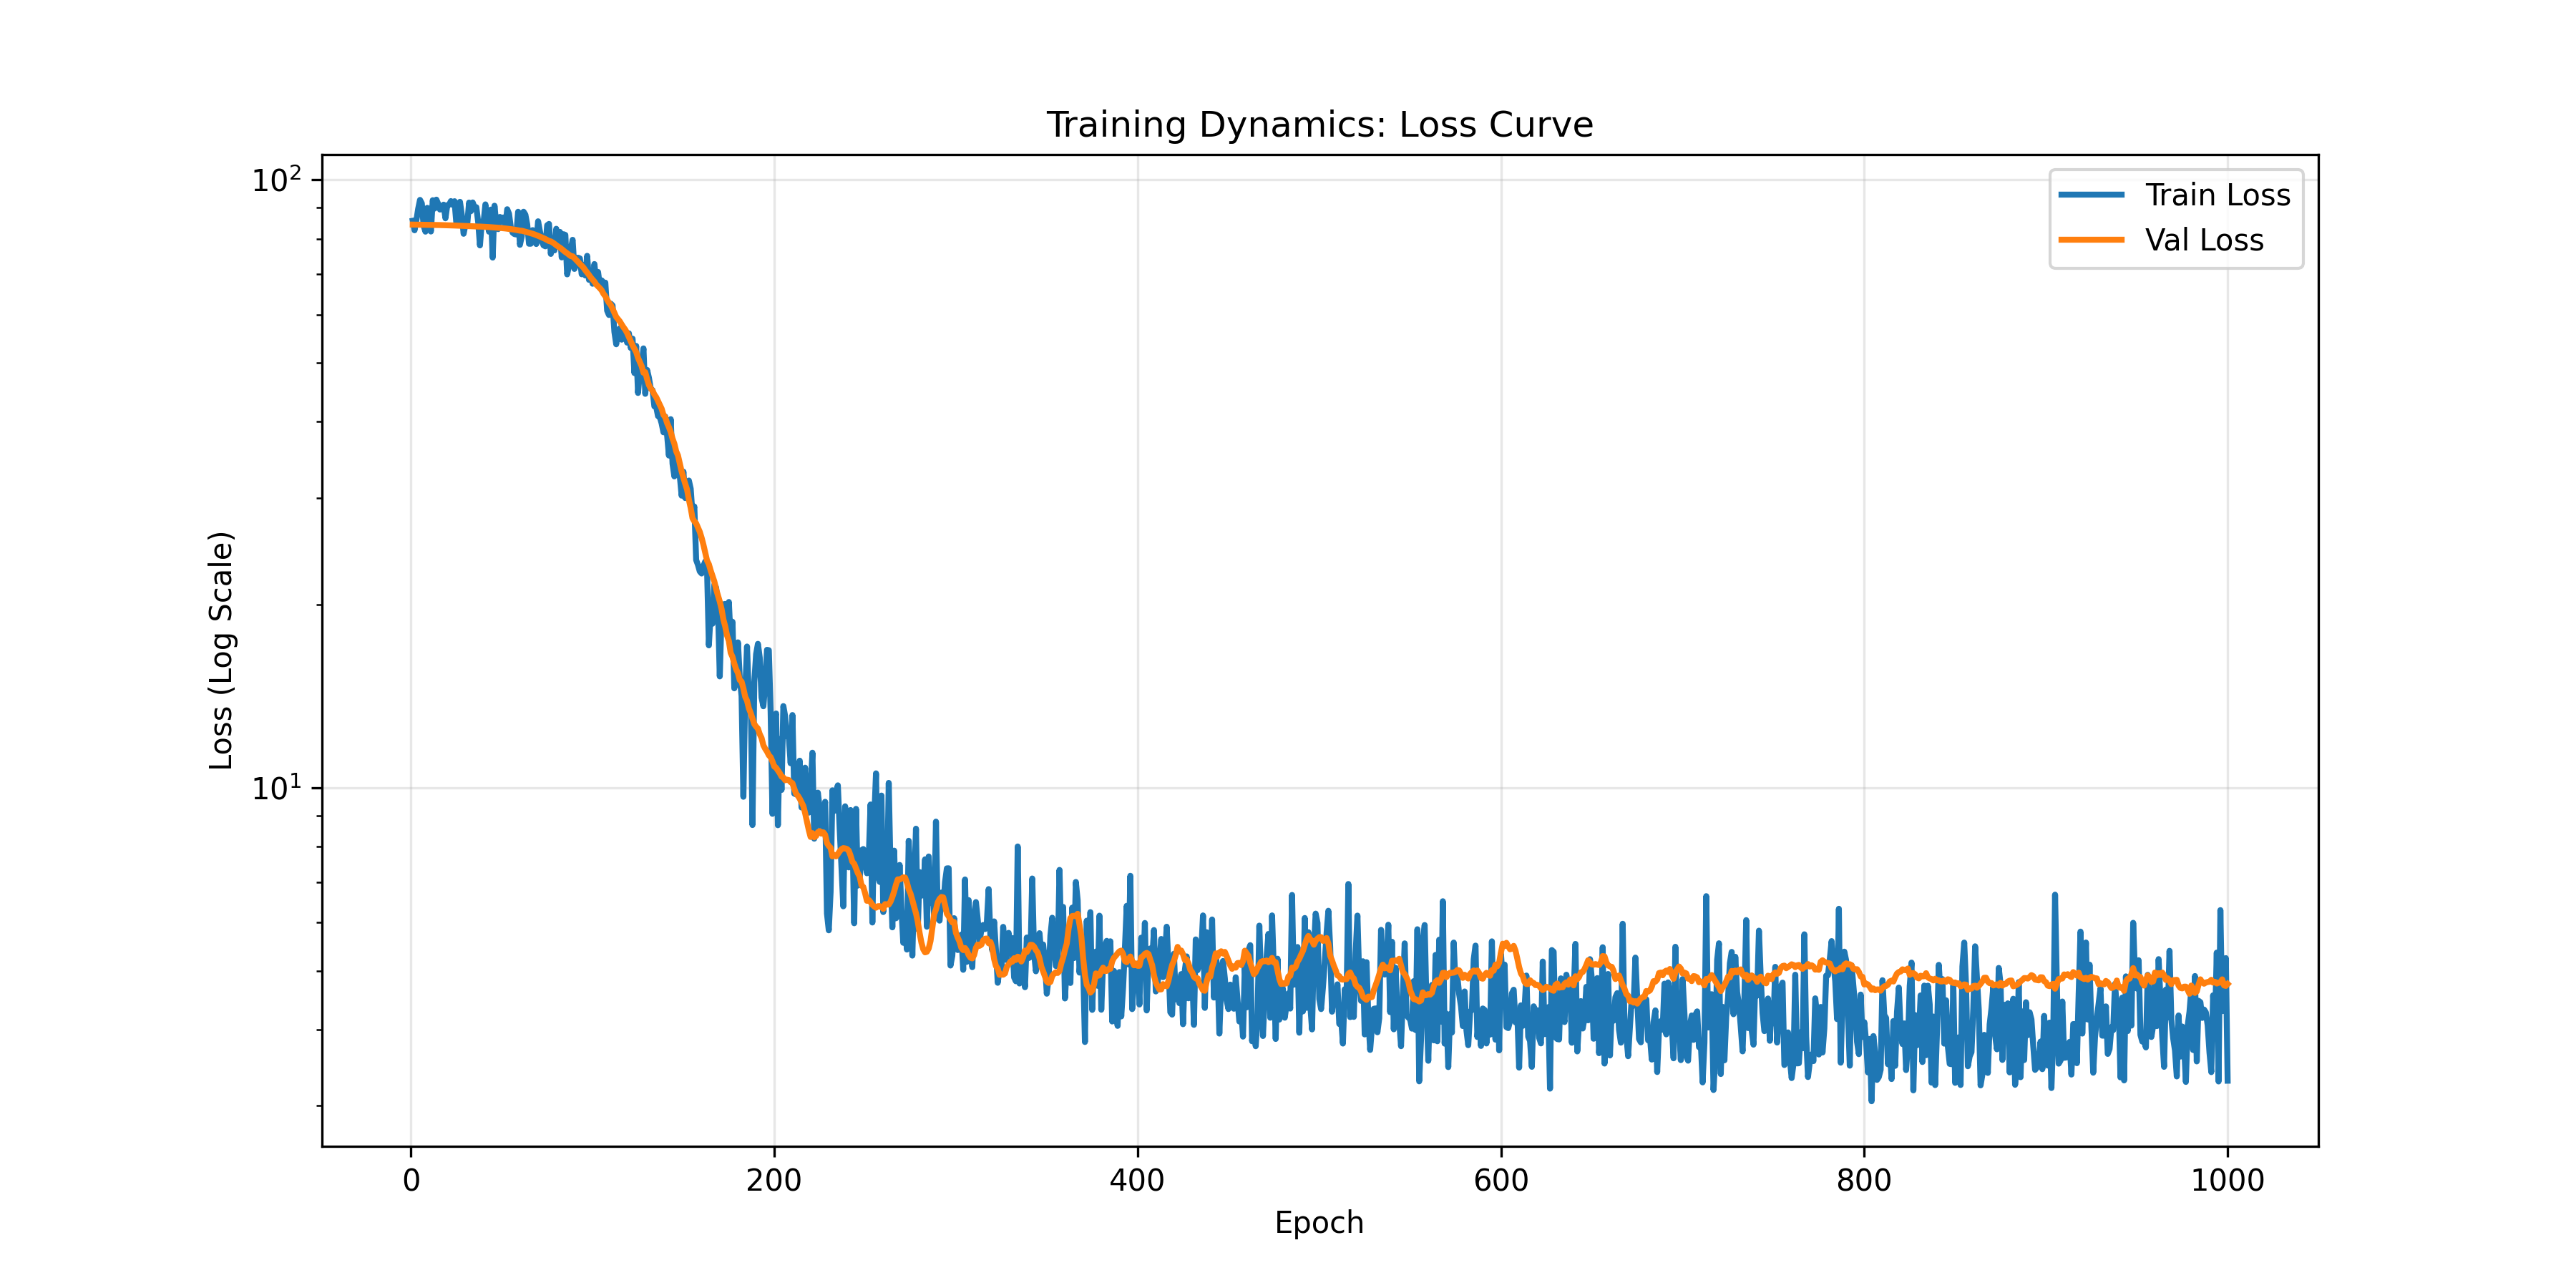
\includegraphics[width=0.9\textwidth, height=0.7\textheight, keepaspectratio]{images/loss_curve.png}
                \caption{Training Convergence (Best Val Loss: 82.45)}
            \end{figure}
        \end{column}
    \end{columns}
\end{frame}

\begin{frame}{The Perplexity}
\begin{figure}
    \centering
    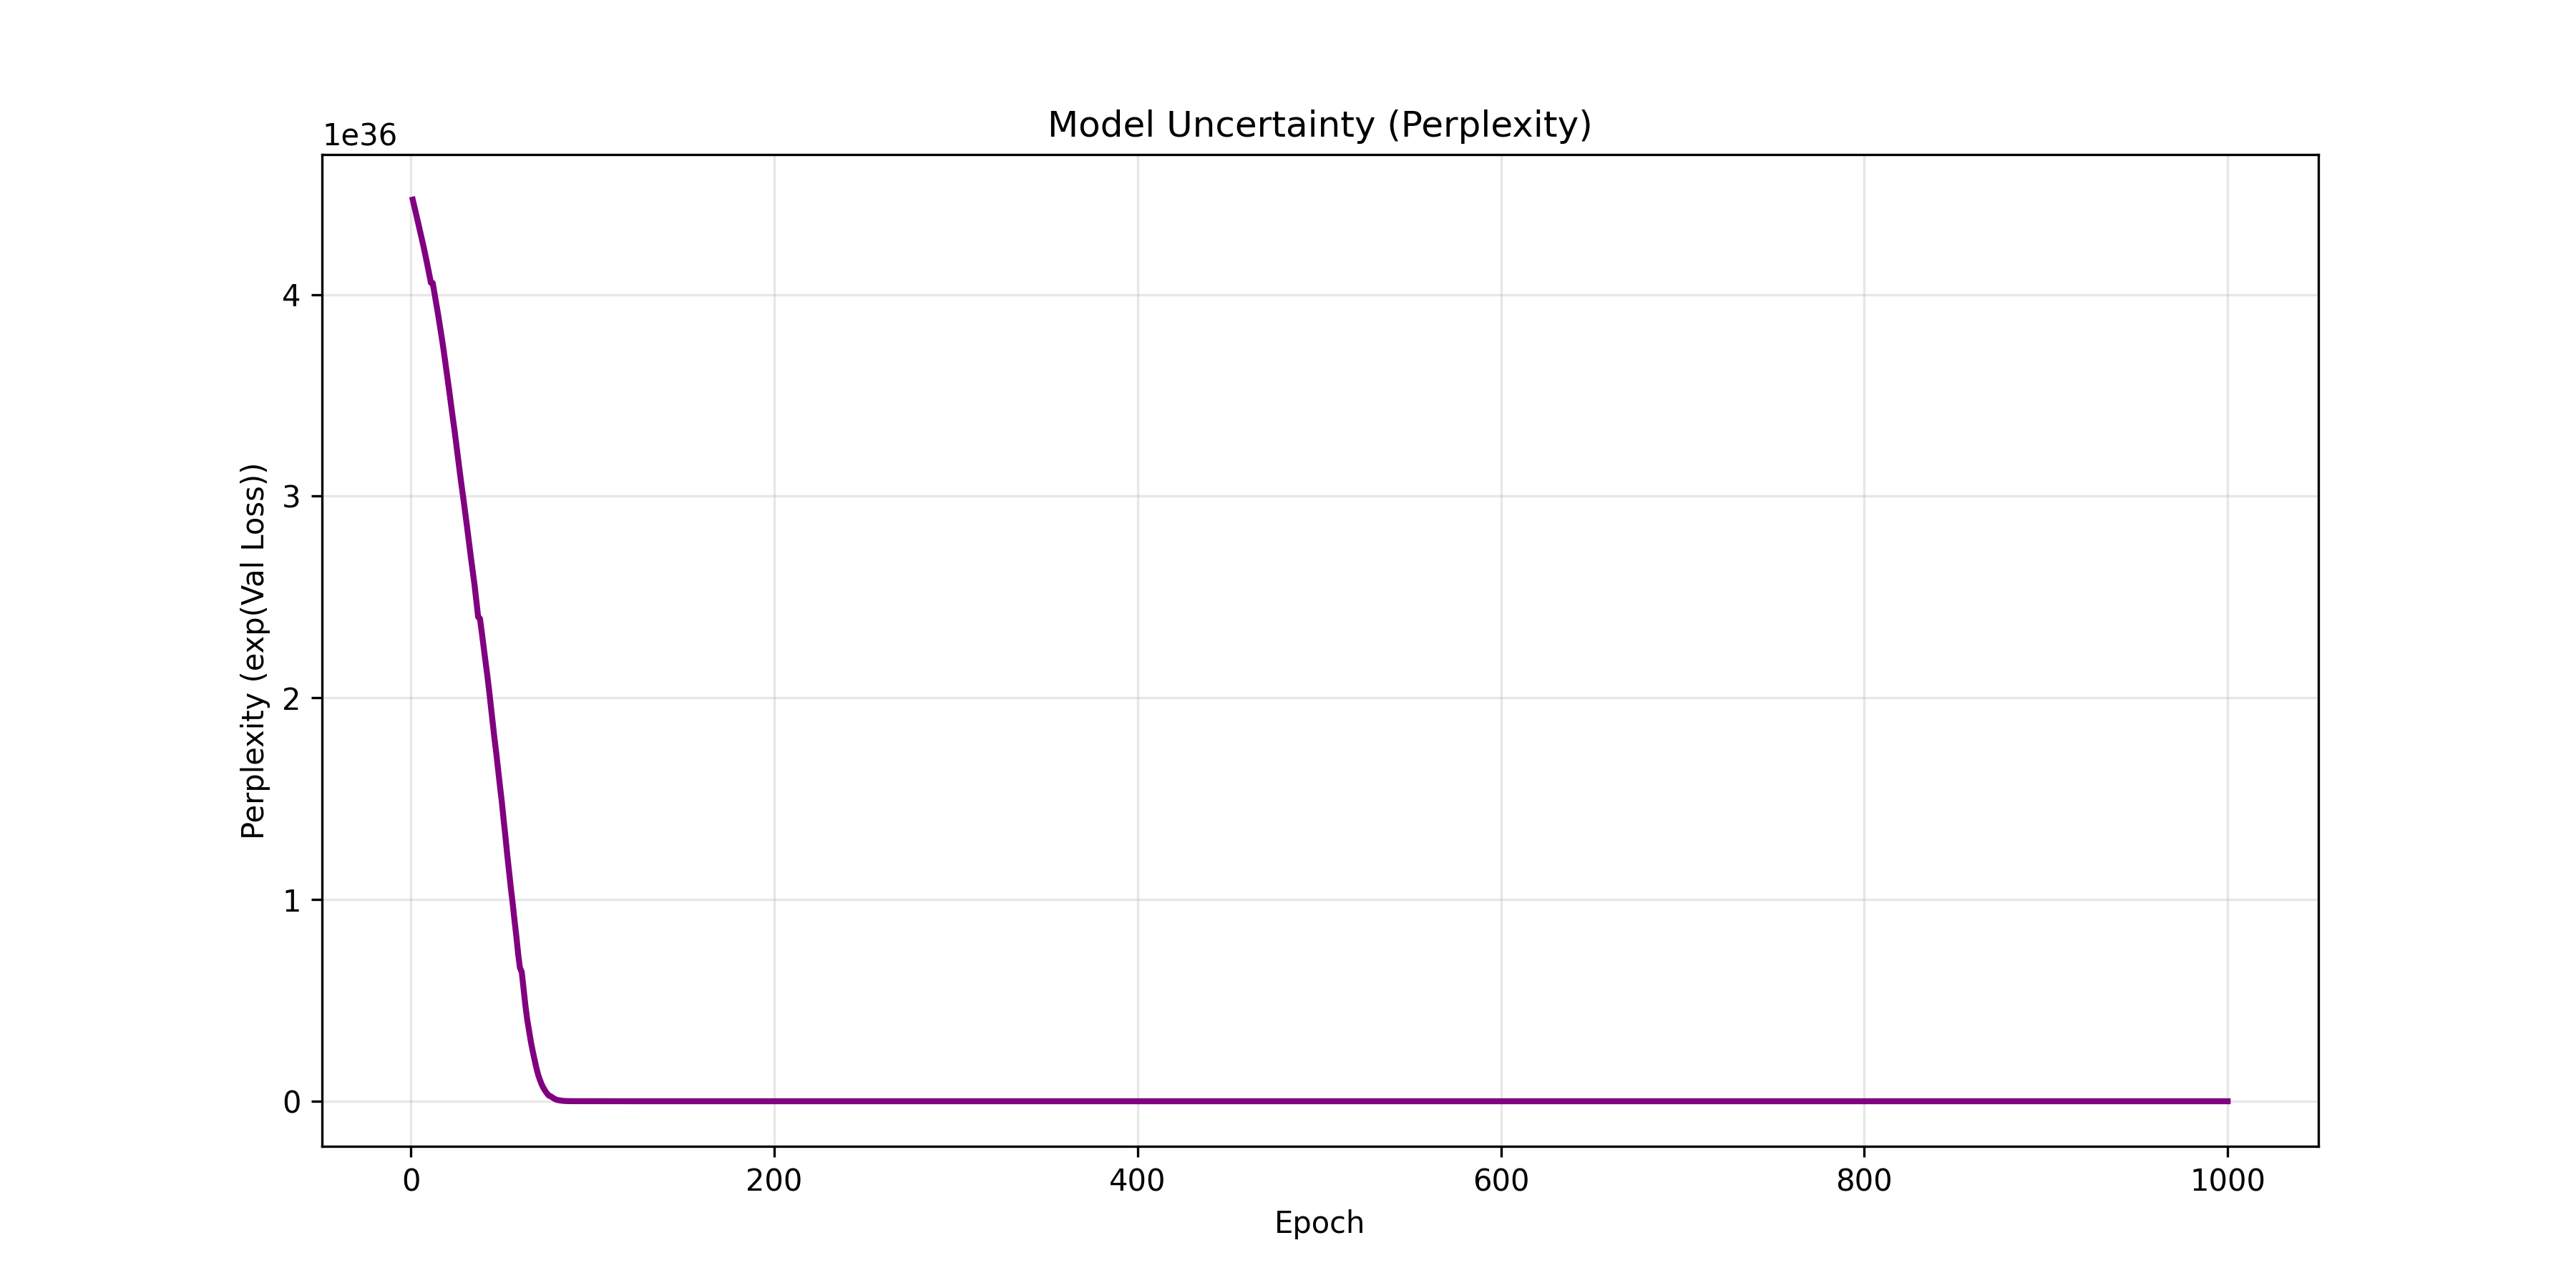
\includegraphics[width=0.5\linewidth]{images/perplexity.png}
    \caption{$\displaystyle 
\mathrm{PPL}=\exp\!\left(-\tfrac{1}{N}\sum_{i=1}^{N}\ln p(x_i)\right)$ 
\; (effective number of equally likely outcomes)
}
    \label{fig:placeholder}
\end{figure}
    
\end{frame}

% --- Section 2: Latent Space Physics ---
\subsection{Latent Space Physics}

\begin{frame}{Discovery: The Latent Response Function}
    We discovered that the learned latent space is not a black box, but a \textbf{physically meaningful manifold}.
    
    \vspace{0.5cm}
    \begin{columns}[T]
        \begin{column}{0.48\textwidth}
            \textbf{1. Geometric Response (Linearity)}
            \begin{itemize}
                \item \textit{Question:} Does the latent vector move linearly as we tune $\epsilon$?
                \item \textbf{Metric:} Correlation between $\epsilon$ and Euclidean distance $d = ||z(\epsilon) - z(0)||_2$.
                \item \textbf{Result:} \textbf{97.55\%}. The model learned a smooth, linear mapping of physics.
            \end{itemize}
        \end{column}
        \begin{column}{0.48\textwidth}
        \begin{figure}
                \centering
                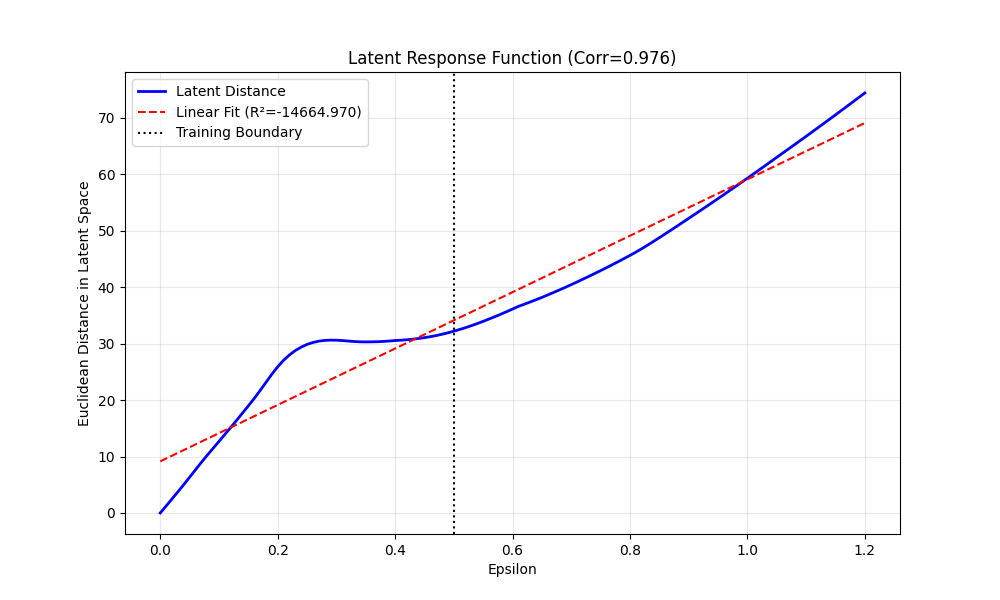
\includegraphics[width=\textwidth, height=0.5\textheight, keepaspectratio]{images/latent_response_function.png}
                \caption{Latent Distance vs. Epsilon ($R^2 \approx 1.0$)}
            \end{figure}
        \end{column}
    \end{columns}
\end{frame}

\begin{frame}{Latent Space Smoothness}
\begin{figure}
    \centering
    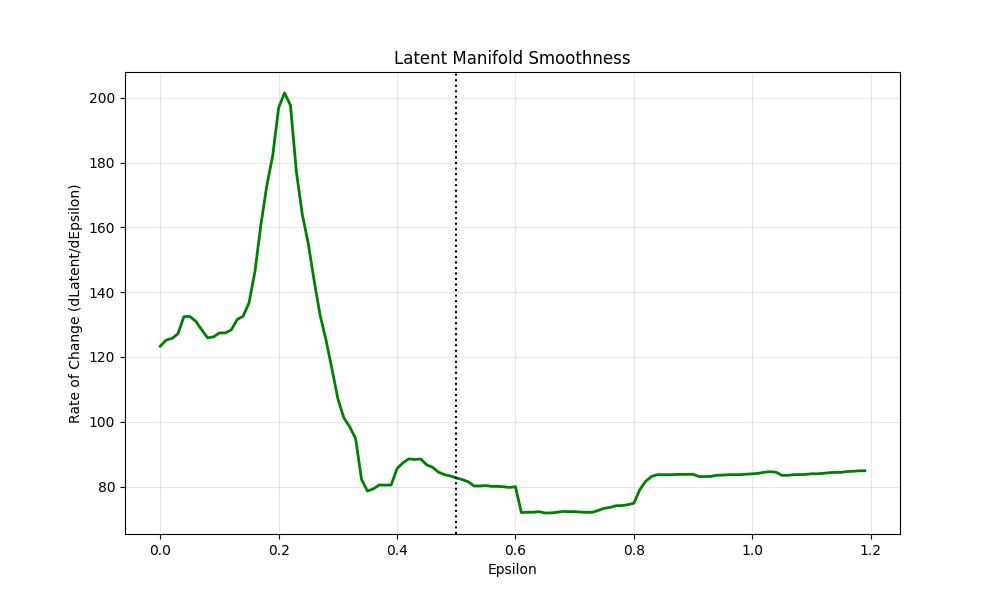
\includegraphics[width=0.9\linewidth]{images/latent_smoothness.png}
    \caption{How the smoothness changes}
    \label{fig:placeholder}
\end{figure}
    
\end{frame}

\begin{frame}{Latent Space Manifold Visualization}
    \begin{figure}
        \centering
        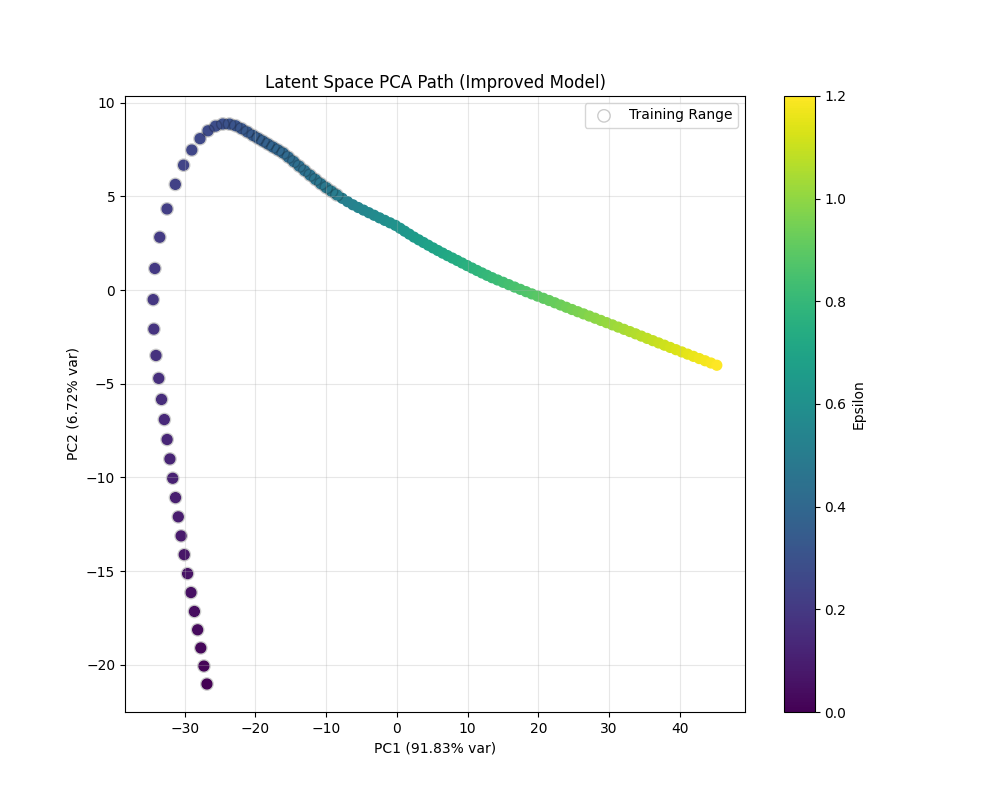
\includegraphics[width=0.65\textwidth, height=0.75\textheight, keepaspectratio]{images/latent_pca_path.png}
        \caption{2D PCA Projection of the Latent Manifold. Note the smooth, continuous trajectory from hydrophobic (purple) to hydrophilic (yellow).}
    \end{figure}
\end{frame}

\begin{frame}{Dynamic Response: "Latent Activity"}
    We defined a new metric, \textbf{Latent Activity}, to measure the "training effort" required for each physical state.
    
    $$ \text{Activity}(\epsilon) = \text{AUC} = \int_{0}^{T} ||z(\epsilon, t)||_2 \, dt $$

    \begin{columns}[T]
        \begin{column}{0.5\textwidth}
            \begin{itemize}
                \item \textbf{Activity (AUC):} Proportional to thermodynamic complexity.
                \item \textbf{Susceptibility ($\chi$):} $\frac{d(\text{Activity})}{d\epsilon}$.
                \item \textbf{Key Finding:} High susceptibility correlates with low Kinetic Energy error (-0.89). The model needs a "responsive" latent space to capture thermal fluctuations.
            \end{itemize}
        \end{column}
        \begin{column}{0.5\textwidth}
        \begin{figure}
                \centering
                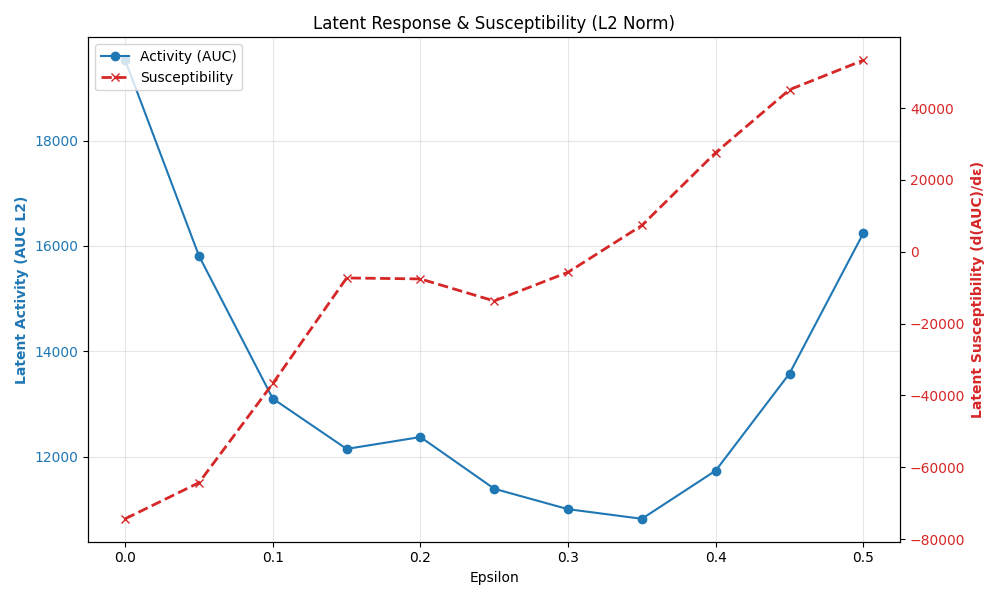
\includegraphics[width=\textwidth, height=0.6\textheight, keepaspectratio]{images/latent_susceptibility_l2.png}
                \caption{Activity and Susceptibility vs. $\epsilon$}
            \end{figure}
        \end{column}
    \end{columns}
\end{frame}

% --- Section 3: Benchmarking Results ---
\section{Results \& Discussion}
\subsection{Benchmarking}

\begin{frame}{Benchmarking: Structural Predictions (RDF)}
    \begin{figure}
        \centering
        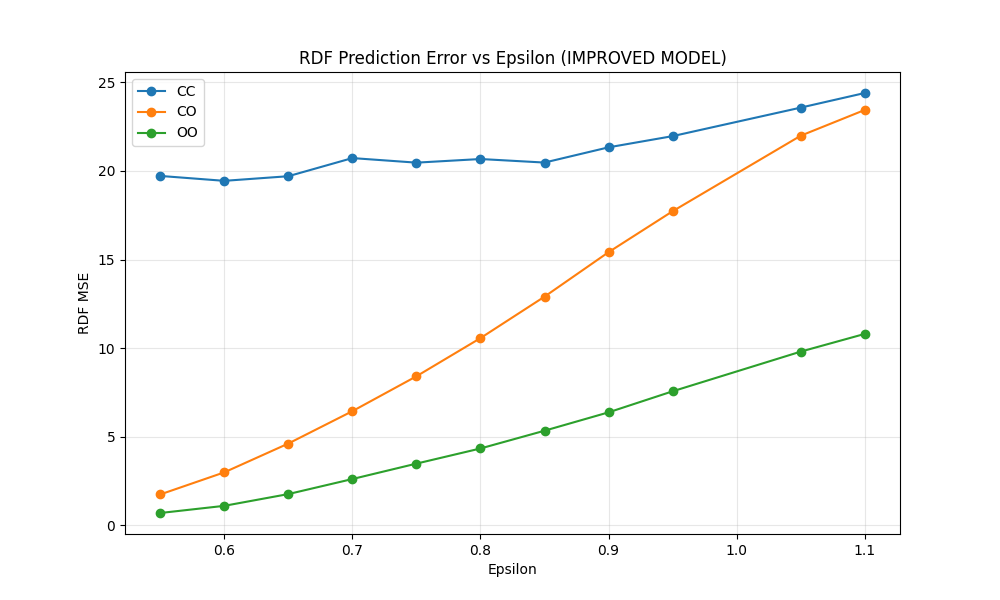
\includegraphics[width=0.9\textwidth, height=0.55\textheight, keepaspectratio]{images/summary_rdf_mse.png}
        \caption{RDF Prediction Error (MSE) across Epsilon Range}
    \end{figure}

    \begin{columns}[T]
        \begin{column}{0.33\textwidth}
            \textbf{C-C (Bulk):}
            \textcolor{green}{Excellent.}
            Correlation increases to 0.77 at high $\epsilon$.
        \end{column}
        \begin{column}{0.33\textwidth}
            \textbf{O-O (Solvent):}
            \textcolor{orange}{Good.}
            Stable until $\epsilon > 0.9$.
        \end{column}
        \begin{column}{0.33\textwidth}
            \textbf{C-O (Interface):}
            \textcolor{red}{Poor.}
            Model struggles with the exact interface structure.
        \end{column}
    \end{columns}
\end{frame}

\begin{frame}{Benchmarking: Thermodynamic Stability}
    \begin{columns}[T]
        \begin{column}{0.5\textwidth}
        \begin{figure}
                \centering
                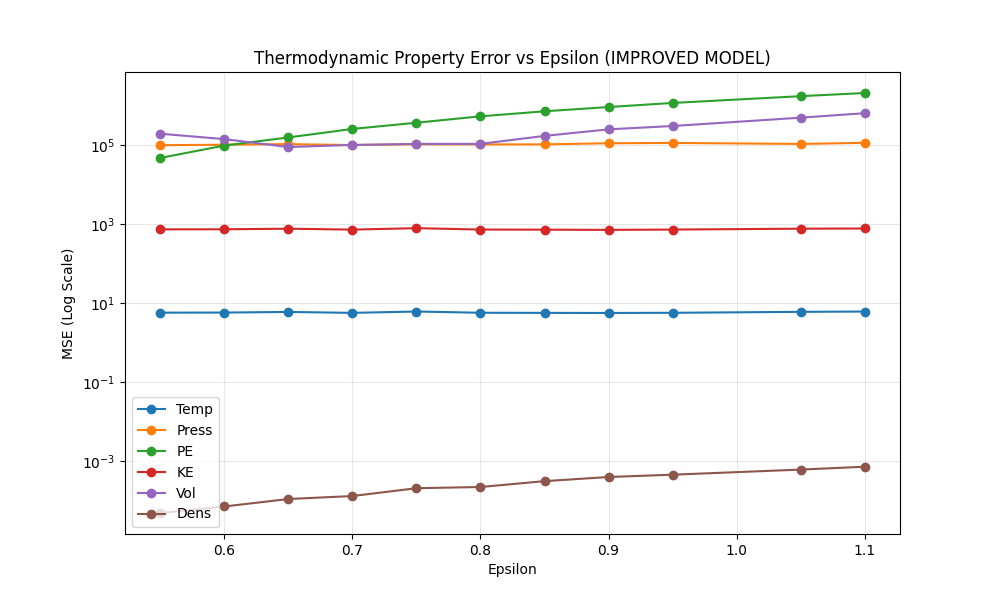
\includegraphics[width=\textwidth, height=0.6\textheight, keepaspectratio]{images/summary_thermo_mse.png}
                \caption{Thermodynamic MSE (Log Scale)}
            \end{figure}
        \end{column}
        \begin{column}{0.5\textwidth}
            \textbf{Safe Operating Range:}
            \begin{itemize}
                \item \textbf{$\epsilon \le 0.70$:} High Confidence. All metrics stable.
                \item \textbf{$\epsilon \le 0.85$:} Production Ready. Structural predictions reliable.
                \item \textbf{$\epsilon > 0.85$:} Extrapolation breakdown. Potential Energy error grows exponentially.
            \end{itemize}
            
            \vspace{0.3cm}
            \textit{Temperature is stable (MSE $\approx$ 6 K$^2$) across the entire range.}
        \end{column}
    \end{columns}
\end{frame}

\begin{frame}{Visual Validation: RDF Comparison ($\epsilon=0.70$)}
    \begin{figure}
        \centering
        % Ensure filename matches what was generated
        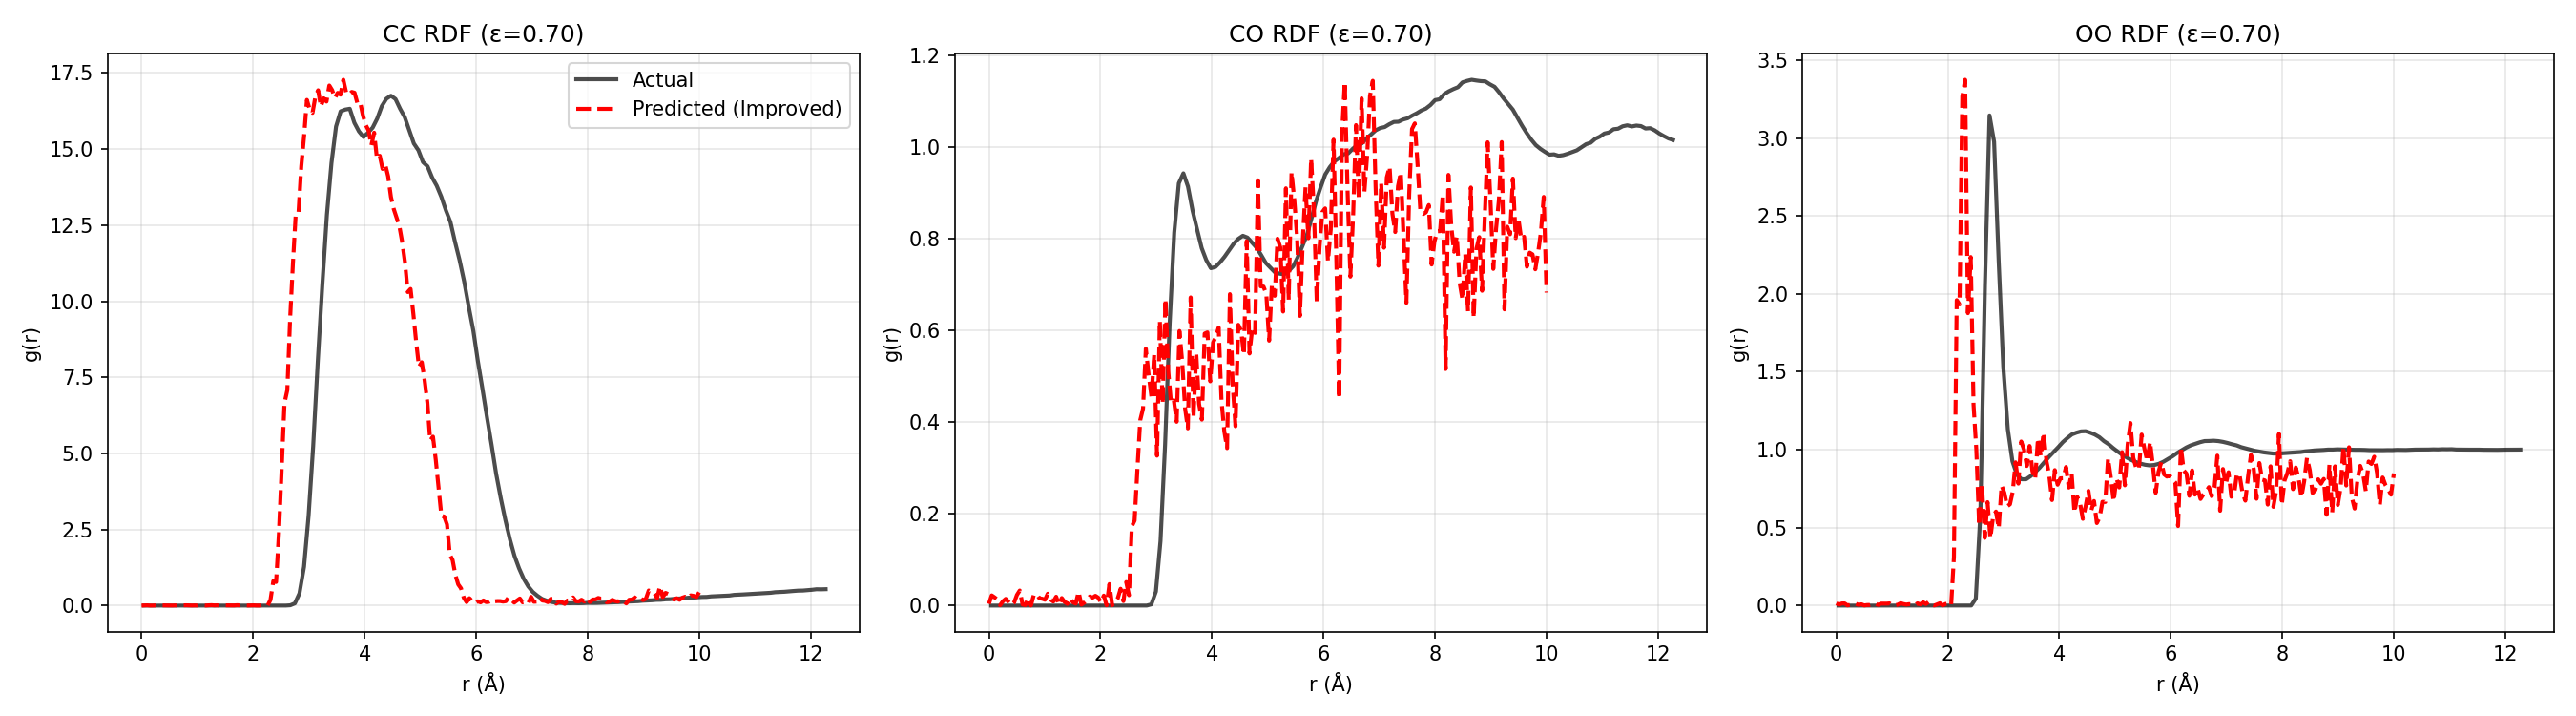
\includegraphics[width=0.95\textwidth, height=0.6\textheight, keepaspectratio]{images/rdf_comparison_eps_0.70.png}
        \caption{Actual (Black) vs. Predicted (Red) RDFs at $\epsilon=0.70$. Note the excellent agreement for C-C peaks.}
    \end{figure}
\end{frame}

% --- Section 4: Conclusion ---
\section{Conclusion \& Future Work}
\subsection{Final Assessment}

\begin{frame}{Final Assessment}
    \begin{block}{Successes}
        \begin{enumerate}
            \item \textbf{Physical Latent Space:} The model didn't just memorize data; it learned a linear physical manifold ($R=0.975$).
            \item \textbf{Structural Generalization:} C-C RDF predictions improve in the extrapolation regime.
            \item \textbf{Efficiency:} 45\% faster training than the baseline.
        \end{enumerate}
    \end{block}

    \vspace{0.5cm}
    \begin{alertblock}{Limitations \& Future Work}
        \begin{itemize}
            \item \textbf{Interface (C-O):} Needs specific attention mechanisms or weighted loss.
            \item \textbf{Energy Extrapolation:} Validity limited to $\epsilon \le 0.85$.
        \end{itemize}
    \end{alertblock}
\end{frame}


\subsection{Future Directions}
\begin{frame}{Future Works:}
\large
\centering
\begin{enumerate}
    \item Complete the MD for more accurate OPLS-AA model of the fullerene 
    \item Try different topologies of molecules/nanoparticles
    \item Generalize the Response Function of the Latent Space of a training session for a model to correlate with the initial real world data it was fed. (Currently in my literature review I couldn't find anything that closely resembles it.
\end{enumerate}
    
\end{frame}

\begin{frame}{Also This!!!}
\begin{figure}
    \centering
    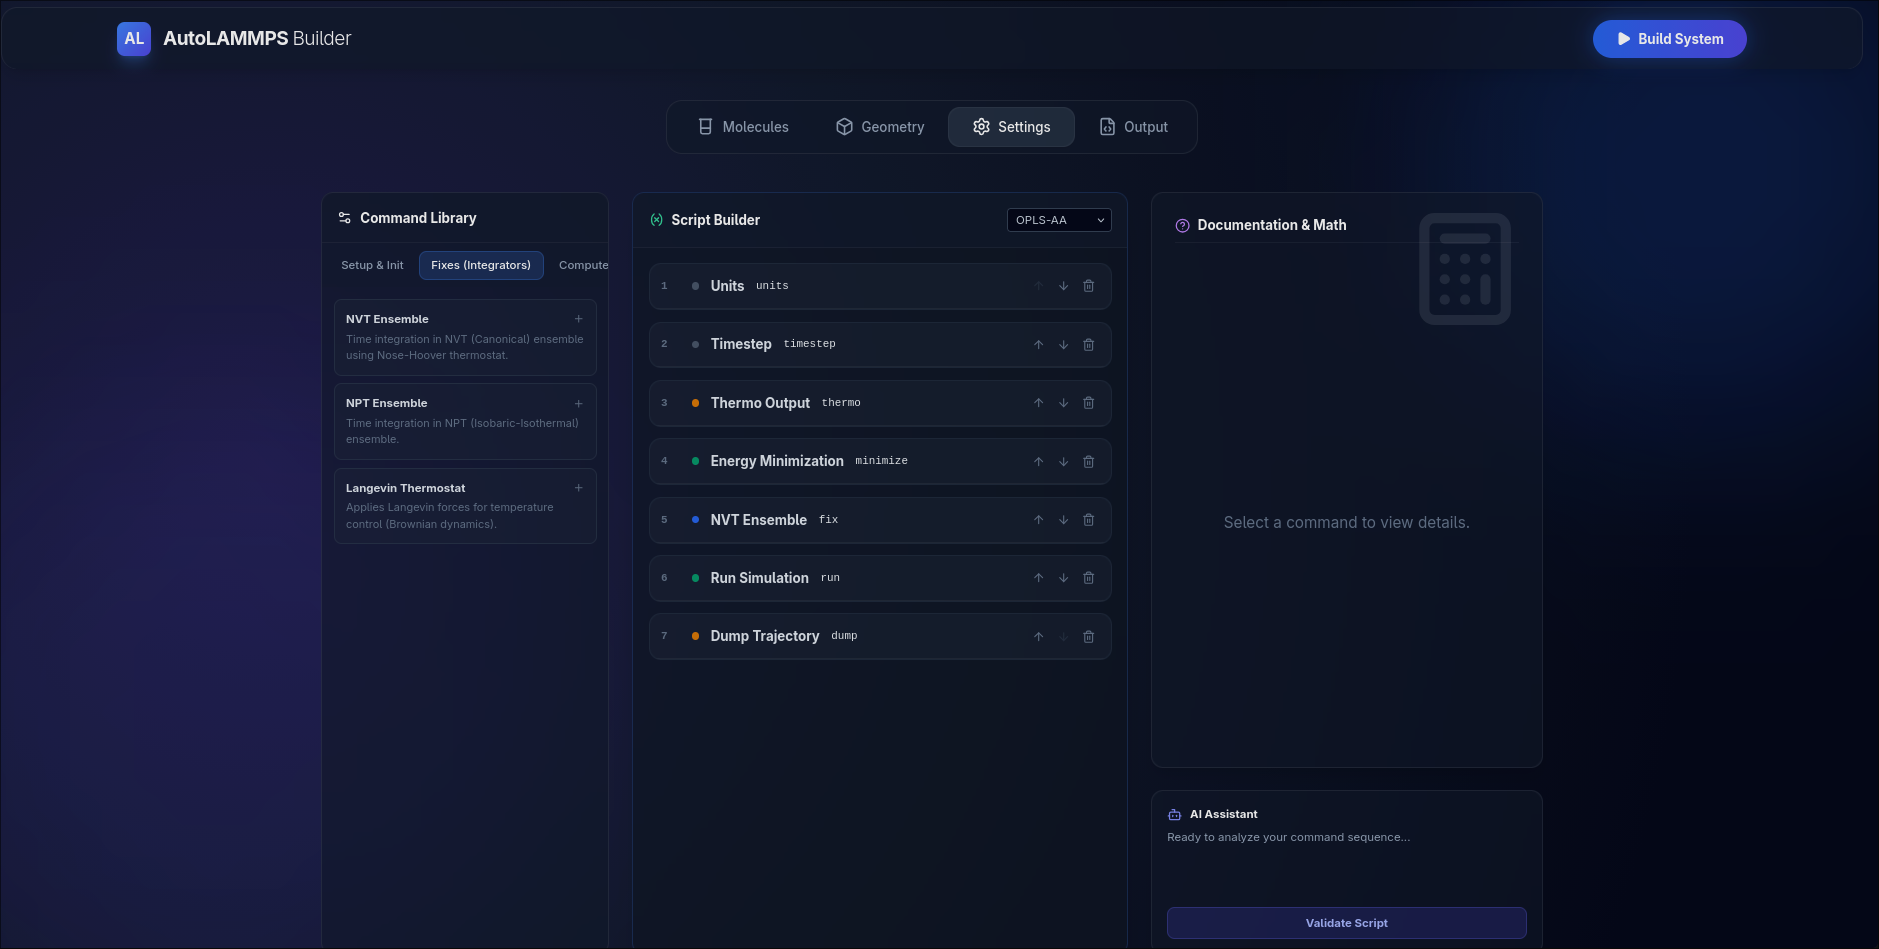
\includegraphics[width=0.9\textwidth, height=0.9\textheight, keepaspectratio]{images/autolammps_script.png}
    \caption{AutoLAMMPS Script}
\end{figure}
\end{frame}

\begin{frame}[allowframebreaks]{References}
    \printbibliography
\end{frame}

\end{document}
